% Nucleus — technical document.
% Build:  nix develop --command just build   (LuaLaTeX + biber via latexmk)
% This document is COHESIVE and STANDALONE: it must not reference
% internal task ids or PRD paragraph numbers anywhere in its prose.
\documentclass[11pt,a4paper,oneside]{memoir}

% Preamble — packages and dissertation styling.
% Engine: LuaLaTeX (fontspec requires lua/xe; the build uses lualatex).

\usepackage{fontspec}            % Unicode/OpenType font handling (LuaTeX).
\usepackage{microtype}           % Micro-typographic refinements.
\usepackage[english]{babel}

\usepackage{graphicx}
\usepackage{booktabs}            % Professional tables.
\usepackage{array}
\usepackage{xcolor}
\usepackage{enumitem}

% --- Figures: TikZ / PGF ---
\usepackage{tikz}
\usetikzlibrary{
  arrows.meta, positioning, fit, calc, shapes.geometric,
  shapes.misc, backgrounds, matrix, chains, decorations.pathreplacing
}
\usepackage{pgfplots}
\pgfplotsset{compat=1.18}

% --- Code listings (Nuc + Rust) ---
\usepackage{listings}
\definecolor{lstkw}{RGB}{20,20,160}
\definecolor{lstcomment}{RGB}{100,100,100}
\definecolor{lststring}{RGB}{160,40,40}
\lstdefinestyle{nuc}{
  basicstyle=\ttfamily\small,
  keywordstyle=\color{lstkw}\bfseries,
  commentstyle=\color{lstcomment}\itshape,
  stringstyle=\color{lststring},
  showstringspaces=false,
  columns=fullflexible,
  breaklines=true,
  frame=single,
  framesep=4pt,
  numbers=left, numberstyle=\ttfamily\scriptsize\color{lstcomment},
}
\lstset{style=nuc}
% A light Nuc-language listing dialect (extend in the language chapter).
\lstdefinelanguage{Nuc}{
  morekeywords={algorithm,schedule,kernel,pure,effectful,worker,workers,
    map,for,repeat,block,vectorize,reuse,pipeline,sync,transfer,buffer,
    check,partition,backend,in,out},
  morecomment=[l]{//},
  morestring=[b]",
}

% --- Bibliography ---
\usepackage{csquotes}            % biblatex-recommended when babel is loaded.
\usepackage[backend=biber,style=numeric-comp,sorting=nyt]{biblatex}

% Verbatim (grammar productions, shell recipes) is set a notch smaller so the
% long BNF/command lines in the appendices fit the text block without spilling
% into the margin. Only affects verbatim environments.
\makeatletter
\renewcommand{\verbatim@font}{\normalfont\ttfamily\footnotesize}
\makeatother

% A break hint for the long German title in the bibliography (Petri 1962),
% which is otherwise unbreakable and overflows the line. LuaTeX takes the
% accented character literally (UTF-8), not as a control sequence.
\hyphenation{Rhei-nisch-West-fä-li-schen}

% --- Cross-references (load hyperref then cleveref last) ---
\usepackage{hyperref}
\hypersetup{
  colorlinks=true,
  linkcolor=black, citecolor=black, urlcolor=blue,
  pdftitle={Nucleus: a deterministic algorithm/schedule co-compiler},
  pdfauthor={Mark Ruvald Pedersen},
}
\usepackage{cleveref}

% Convenience macros.
\newcommand{\nuc}{\textsc{Nucleus}}
\newcommand{\nuclang}{\textsc{Nuc}}
% \todo renders nothing: the draft is content-complete and no TODO marker
% should reach an examiner. Kept as a defined no-op so any stray call is
% silent rather than a build error or red ink.
\newcommand{\todo}[1]{}

% Tier-1 differential-matrix totals, sourced from the live e2e harness
% (single source of truth so prose and tables cannot disagree). Verified
% against a clean `nucleus-e2e` run: total / pass / skipped (fail = 0).
\newcommand{\nmatrixtotal}{483}
\newcommand{\nmatrixpass}{420}
\newcommand{\nmatrixskip}{63}

\addbibresource{refs.bib}

\title{\nuc: A Deterministic Algorithm/Schedule Co-Compiler with\\
       First-Class IO Semantics and a Petri-Net Soundness Gate}
\author{Mark Ruvald Pedersen}
\date{\today}

\begin{document}

\frontmatter
% Title page. A formal dissertation title block.
\begin{titlingpage}
\centering
\vspace*{2cm}
{\Huge\bfseries \nuc\par}
\vspace{0.6cm}
{\Large A Deterministic Algorithm/Schedule Co-Compiler with\\[0.2em]
 First-Class IO Semantics and a Petri-Net Soundness Gate\par}
\vfill
{\large A dissertation submitted for the degree of\\ Doctor of Philosophy\par}
\vspace{1.5cm}
{\large\bfseries Mark Ruvald Pedersen\par}
\vfill
{\large \today\par}
\end{titlingpage}

% Declaration omitted: this is a technical document, not a degree submission.
% Abstract. ~250 words. Every number here is grounded in the implementation.
\chapter*{Abstract}
\addcontentsline{toc}{chapter}{Abstract}

Portable parallel software couples three concerns that ought to be separable:
the \emph{algorithm} (what to compute), its \emph{decomposition and IO} (how to
lay it out across workers in space and time, and with what IO semantics), and
the \emph{target platform}. Moving an algorithm from CPU threads to a
message-passing cluster to an embedded microcontroller today means rewriting it,
because decomposition and IO semantics are written by hand, per platform, and
tangled into the source. Compute scheduling has first-class language support;
IO scheduling does not.

This dissertation presents \nuc, a source-to-source compiler --- it emits Rust
that a downstream host toolchain builds --- founded on a strict separation
between an algorithm sublanguage and a schedule sublanguage. Decomposition, IO
semantics (synchronous or asynchronous, buffered or unbuffered, event-driven or
polled, shared-memory or message-passing or DMA), and target are first-class
schedule directives that the algorithm never sees: one algorithm composes with
many schedules, and each schedule composes with many backends. A single
Petri-net intermediate representation unifies transfer synthesis,
synchronisation, and a compile-time soundness gate, so boundedness and
deadlock-freedom are reported as compile errors rather than runtime surprises.
The genericity claim is made mechanically falsifiable by a cross-backend
bit-identical differential test: the same algorithm, under every schedule and
backend, must produce byte-identical output.

The implementation drives twenty-seven worked examples through ten backends
across three tiers --- seven shared-memory and message-passing CPU backends, two
MPI backends, and one embedded backend with multi-microcontroller co-simulation.
The seven CPU backends agree byte-for-byte across the full schedule-by-backend
matrix; the embedded backend reproduces reference output byte-exactly under
co-simulation. The work is honest about its boundary: the algorithm class is
affine, static, single-assignment, and integer-valued, and the schedule is
checked, not optimised.

% Acknowledgements omitted: this is a technical document, not a degree thesis.
\cleardoublepage
\tableofcontents
\listoffigures
\listoftables

\mainmatter
\chapter{Introduction}\label{ch:introduction}
% Content cycle: C2. Intent: state the portability problem; motivate the
% algorithm/schedule split; give the thesis statement + contributions; bound
% the scope (the algorithm class); lay out the dissertation structure.

\section{The portability problem}\label{sec:intro-problem}
% Porting an algorithm across CPU threads / MPI cluster / embedded MCU means
% rewriting it: decomposition + IO semantics are hand-written, per platform.

\section{Motivation}\label{sec:intro-motivation}
% IO is a second-class citizen (compute scheduling has Halide/TVM/Exo; IO
% does not); hardware churns faster than algorithms; decomposition is the
% expensive, error-prone part.

\section{Thesis statement and contributions}\label{sec:intro-contributions}
% Algorithm/schedule separation; IO as a first-class schedule directive; one
% Petri-net IR with a compile-time soundness gate; falsifiable genericity via
% a cross-backend bit-identical differential test.

\section{Scope and non-goals}\label{sec:intro-scope}
% The affine/static/single-assignment algorithm class; what is deliberately
% out (data-dependent writes, recursion, dynamic scheduling).

\section{Structure of this dissertation}\label{sec:intro-structure}

\todo{Write Chapter 1 (cycle C2).}

\chapter{Background}\label{ch:background}

This chapter introduces the concepts the rest of the document depends on. It
is deliberately neutral: it presents established ideas --- separation of
concerns in parallel programming, the dimensions of IO semantics, static versus
dynamic scheduling, Petri nets, and differential testing --- without yet
assuming the contribution. A reader already fluent in any of these sections may
skip it.

\section{Parallel decomposition and separation of concerns}\label{sec:bg-decomp}

A sequential program states \emph{what} to compute. A parallel program must also
state \emph{how} the work is divided across processing elements and \emph{how}
those elements coordinate. These are different concerns, and conflating them is
the source of much of the difficulty in parallel programming: a change to the
data layout for one machine forces edits all through code that expresses the
mathematics, and the mathematics becomes hard to read through the layout.

The decomposition itself has two axes. \emph{Spatial} decomposition divides data
or iterations across workers that run concurrently --- domain decomposition of a
grid, blocking of a matrix, partitioning of an array. \emph{Temporal}
decomposition orders work within a worker and overlaps it across workers ---
loop tiling, software pipelining (overlapping successive loop iterations so
workers stay busy), and double buffering (alternating between two buffers so a
producer can fill one while the consumer drains the other). Both axes are
scheduling decisions: they change performance and resource use, but, applied
correctly, they do not change the computed result.

The idea that the result-defining part of a program should be written once and
the performance-defining part chosen separately has a clear lineage in
high-performance compute. Halide~\cite{ragan-kelley2013halide} crystallised it
as the explicit split between an \emph{algorithm} (pure functions over an index
domain) and a \emph{schedule} (the tiling, fusion, vectorisation, and
parallelism applied to it), and showed that a single algorithm could be
retargeted across schedules by orders of magnitude in performance without
touching its definition. The polyhedral
compilers~\cite{baghdadi2019tiramisu,bondhugula2008pluto} pursue the same
separation through a more powerful mathematical model. What unites them is the
discipline that the algorithm never mentions the schedule. This document
adopts that discipline and extends it from scheduling computation \emph{within a
single machine} (intra-node) to decomposition and IO \emph{across many machines
or workers} (inter-node). A middle ground between fully manual and fully
automatic decomposition is to have the programmer annotate the decomposition
explicitly --- in a separate schedule sublanguage --- while leaving the compiler
to infer the resulting transfers from those annotations; that is the approach
taken here and developed in \cref{ch:language}.

\section{IO semantics as a programming concern}\label{sec:bg-io}

When two workers exchange data, the exchange is governed by choices that are
usually made implicitly by whatever runtime is in use, but which materially
affect correctness and performance. These choices form a small set of orthogonal
dimensions:

\begin{description}[leftmargin=*]
  \item[Synchronous vs.\ asynchronous.] Does the producer block until the
        transfer completes, or does it initiate the transfer and continue,
        completing it later? Asynchrony enables latency hiding but requires
        somewhere to track the in-flight operation.
  \item[Buffered vs.\ unbuffered.] Is there storage that decouples producer and
        consumer rates, allowing the producer to run ahead by a bounded number
        of items, or must each transfer rendezvous directly?
  \item[Event-driven vs.\ polled.] Is the consumer woken when data arrives (by
        an interrupt, a condition variable, or an event-loop readiness
        notification), or does it repeatedly test for arrival?
  \item[Transport.] Do the bytes move through shared memory, a loopback or
        network socket, a Unix domain socket, a cluster interconnect via a
        message-passing library, or a DMA engine on an embedded device?
\end{description}

These dimensions are largely independent of one another and of the algorithm. A
shared-memory threads runtime such as OpenMP~\cite{dagum1998openmp} fixes one
combination; a message-passing library such as MPI~\cite{mpiforum2021} offers
several (blocking and non-blocking sends, buffered and synchronous modes) but
within its own model; an embedded async framework such as
Embassy~\cite{embassy} fixes yet another around interrupts and DMA. Crucially,
none of them lets these choices be \emph{stated} as part of a schedule and
\emph{swapped} without rewriting the communication code. That gap --- IO
semantics as an unspoken property of the chosen runtime rather than a
first-class, selectable directive --- is the gap this work targets.

\section{Static versus dynamic scheduling}\label{sec:bg-scheduling}

A \emph{schedule} assigns operations to workers and orders them in time.
Scheduling may happen dynamically, at run time --- as in work-stealing thread
pools or dataflow runtimes that fire operations when their inputs become
available --- or statically, at compile time, fixing the order before the
program runs.

Dynamic scheduling adapts to data-dependent and machine-dependent variation, at
the cost of runtime overhead, nondeterminism, and analyses that can only be
approximate. Static scheduling gives up that adaptivity but gains three
properties this work depends on. First, \emph{determinism}: a fixed firing order
means a fixed result and a fixed communication pattern, which is what makes
byte-identical cross-backend comparison meaningful. Second,
\emph{analysability}: with the order known at compile time, properties such as
buffer sufficiency and freedom from deadlock become decidable by replaying that
one order, rather than searching a reachable state space. Third, \emph{suitability
for embedded real-time targets}, where dynamic scheduling is often unacceptable
regardless. Static scheduling of dataflow has a long pedigree --- synchronous
dataflow~\cite{lee1987sdf} schedules a restricted graph entirely at compile time
precisely to remove runtime overhead --- and this work sits firmly in that
static tradition. The scope restrictions stated in \cref{sec:intro-scope} ---
affine bounds, single-assignment arrays, and a statically fixed decomposition ---
are exactly what place this work in the static-scheduling camp and make the
analyses of the following sections tractable.

\section{Petri nets}\label{sec:bg-petri}

A Petri net~\cite{petri1962kommunikation,murata1989petri} is a bipartite
directed graph with two kinds of node: \emph{places} and \emph{transitions}.
Places hold \emph{tokens}; a marking is an assignment of a token count to every
place. A transition is \emph{enabled} when each of its input places holds enough
tokens, and \emph{firing} it removes tokens from its input places and deposits
tokens on its output places, producing a new marking. The net's behaviour is the
set of markings reachable from an initial marking by firing enabled transitions.

A handful of standard properties characterise such a net. A net is
\emph{bounded} if no place can ever exceed a stated token capacity, and
\emph{$k$-bounded} if that capacity is $k$. It is \emph{live} if no transition is
permanently disabled. A \emph{deadlock} is a reachable marking in which no
transition is enabled --- the system cannot make progress. For general Petri
nets these properties are decidable but expensive; for restricted subclasses
they become cheap.

Petri nets are a natural model for the problem at hand because their vocabulary
maps directly onto statically scheduled communication. A transition models a
kernel firing, a data transfer, or a synchronisation; a place models a data
slot, a communication channel, or a barrier; a token models the presence of a
value or a unit of buffer credit; a place's capacity models a declared buffer
size; and tokens placed on a channel in the initial marking model the
head-start that double-buffering or software-pipelining provides. Under this
mapping, ``does this schedule's communication stay within its declared
buffers?'' is exactly boundedness, and ``can this schedule's communication
hang?'' is exactly the reachability of a deadlocked marking.
\Cref{ch:architecture} shows how restricting the net to a statically determined
firing order collapses these checks to a single deterministic replay.

\section{Determinism and differential testing}\label{sec:bg-determinism}

\emph{Differential testing}~\cite{mckeeman1998differential} establishes
confidence in a system by comparing the outputs of multiple implementations that
are supposed to agree: where they differ, at least one is wrong, and the
disagreement localises the fault. It is especially powerful for compilers, where
an oracle for ``the correct output'' is otherwise hard to obtain; the
Csmith~\cite{yang2011csmith} work famously used differential testing across C
compilers to find hundreds of bugs by generating programs whose output every
correct compiler must agree on.

Differential testing requires a deterministic notion of agreement. Two
implementations can only be compared byte-for-byte if both are deterministic for
the same input. This is why the algorithm class in this work is restricted to
deterministic arithmetic (\cref{sec:intro-scope}): integer computation, or
floating-point computation whose reductions do not reorder, guarantees that a
single reference output exists for every example. Given that determinism,
differential testing becomes a means not only of finding bugs but of
\emph{falsifying a design claim}. If one algorithm is compiled under many
schedules and many backends and all outputs are byte-identical to a single
hand-written reference, then the claim that the algorithm is independent of
schedule and backend has survived a concrete attempt to break it; a single
differing byte refutes it. \Cref{ch:validation} develops this rig in full.

\chapter{Prior Art and Literature Study}\label{ch:prior-art}
% Content cycle: C2. Intent: survey the field, position the contribution, and
% draw the line to the author's own earlier work. Real BibTeX citations only.

\section{Compute schedulers}\label{sec:pa-compute}
% Halide, TVM, Tiramisu, Exo: compute scheduling is first-class; IO is not.

\section{Parallel runtimes and models}\label{sec:pa-runtimes}
% MPI, OpenMP, Embassy: per-platform, hand-written IO.

\section{Polyhedral compilation}\label{sec:pa-polyhedral}
% isl and the power/cost trade-off versus the affine line drawn here.

\section{Petri-net and dataflow scheduling}\label{sec:pa-petri}

\section{From the 2013 prototype to this work}\label{sec:pa-v1}
% The earlier single-target ISP-firmware prototype: what it sketched, why its
% genericity claim could not be falsified, and the delta this work realises.

\section{Positioning}\label{sec:pa-positioning}
% The specific gap Nucleus fills.

\todo{Write Chapter 3 (cycle C2).}

\chapter{Problem Statement and Solution Space}\label{ch:problem}
% Content cycle: C3. Intent: state the gap precisely, survey the design space,
% and justify the central commitments before any implementation detail.

\section{The portability gap, precisely}\label{sec:prob-gap}

\section{The design space}\label{sec:prob-design-space}
% Where can decomposition + IO live? Trade-offs of each choice.

\section{The central commitment: algorithm/schedule separation}\label{sec:prob-split}
% One algorithm, many schedules; one schedule, many backends.

\section{Why a single Petri-net IR}\label{sec:prob-petri-ir}
% One model carrying transfers, synchronisation, and soundness.

\section{Design commitments and deliberate non-goals}\label{sec:prob-commitments}
% The restrictions that make the genericity claim falsifiable.

\todo{Write Chapter 4 (cycle C3).}

\chapter{The \nuclang{} Language}\label{ch:language}
% Content cycle: C3. Intent: present the two sublanguages by example; show the
% boundary is real; state precisely what cannot be expressed and why.

\section{Two sublanguages, one name table}\label{sec:lang-two}

\section{The algorithm sublanguage}\label{sec:lang-algorithm}
% Shape-typed Rust kernels, dataflow, iteration, pure/effectful, single
% assignment (no aliasing by construction).

\section{The schedule sublanguage}\label{sec:lang-schedule}
% Workers, mapping, blocking/tiling, reuse/pipeline, IO semantics, check.

\section{A worked example: one algorithm, many schedules}\label{sec:lang-example}

\section{What the language cannot express, and why}\label{sec:lang-limits}
% Data-dependent writes (scatter), convergence-driven termination, recursion.

\todo{Write Chapter 5 (cycle C3).}

\chapter{Architecture and Methodology}\label{ch:architecture}
% Content cycle: C3. Intent: walk the compilation pipeline end to end; defend
% the two boundaries; explain the soundness gate and why it is sound here.

\section{The compilation pipeline}\label{sec:arch-pipeline}
% parse -> typed algorithm IR -> link -> ACFG -> transforms -> transfer/halo
% inference -> Petri-net IR -> soundness gate -> per-worker projection ->
% presentation-layer codegen. (Central figure.)

\section{The two boundaries}\label{sec:arch-boundaries}
% Algorithm/schedule; middle-end/presentation.

\section{Algorithm IR and linking}\label{sec:arch-link}

\section{The ACFG and its transforms}\label{sec:arch-acfg}
% vectorise, block, pipeline, reuse.

\section{Transfer and halo inference}\label{sec:arch-transfer}
% Automatic transfer synthesis, not automatic parallelism extraction.

\section{The Petri-net IR and the event contract}\label{sec:arch-petri}

\section{The soundness gate}\label{sec:arch-gate}
% Boundedness, deadlock, conflict-freedom by exact replay over the
% deterministic firing order; why this is sound for the restricted class.

\section{Per-worker projection}\label{sec:arch-projection}
% worker -> ordered EventList.

\section{Presentation-layer codegen}\label{sec:arch-codegen}

\todo{Write Chapter 6 (cycle C3).}

\chapter{Backends and the Target Ladder}\label{ch:backends}
% Content cycle: C3. Intent: show the same EventList realised across three
% tiers; defend backend orthogonality and the capability matrix.

\section{The capability matrix and backend orthogonality}\label{sec:be-matrix}

\section{Tier 1 --- CPU}\label{sec:be-tier1}
% The seven CPU backends; the falsification rig.

\section{Tier 2 --- HPC clusters}\label{sec:be-tier2}
% MPI blocking and non-blocking; SPMD rank dispatch.

\section{Tier 3 --- Embedded}\label{sec:be-tier3}
% no_std, DMA/IRQ shims, multi-MCU co-simulation.

\section{Adding a backend: cost classes and the shim model}\label{sec:be-cost}

\todo{Write Chapter 7 (cycle C3).}

\chapter{A Compilation, End to End}\label{ch:walkthrough}
% Inserted after the Backends chapter; chapter numbering is label-based, so
% downstream chapters renumber automatically. Content cycle: C10.
% Part 1 (this file, sections up to the EventList) traces one program from
% source through every IR stage to the per-worker event lists. Part 2 (the
% backend-lowering sections) shows the same event lists rendered to three
% backends.

The previous chapters described the language, the pipeline, and the backends one
concern at a time. This chapter puts them together. It takes a single program ---
the $3\times3$ stencil of \cref{lst:algo} under the distributed schedule of
\cref{lst:sched}, already familiar from \cref{sec:lang-example} --- and follows it
through every stage of the compiler, from the two source files to the per-worker
event lists and then, in the second half, to generated code on three different
backends. Nothing here is new machinery; everything is a concrete instance of a
pass defined in \cref{ch:architecture}. The purpose is to make the abstract
pipeline legible by watching one program move through it, with the actual
intermediate forms shown at each step.

The stencil is a good specimen because it is small enough to draw in full yet
exercises the parts of the compiler that do real work: it has a neighbourhood
access pattern that forces halo inference, an outer loop that is partitioned across
workers, an inner loop that is both tiled and reuse-optimised, and two transfers
with different IO semantics. Every figure and every intermediate form in this
chapter was produced by the shipping compiler on this exact input; the generated
code in the second half is reproduced from its output verbatim.

\section{The two inputs}\label{sec:wt-inputs}

Recall the division of labour. The algorithm file (\cref{lst:algo}) declares two
$16\times16$ arrays of 32-bit integers, \texttt{img\_in} and \texttt{img\_out};
three kernels --- a side-effecting (\emph{effectful}) \texttt{load\_image}, a pure
\texttt{blur3} taking nine neighbours, and an effectful \texttt{save\_image} (the
purity distinction is made precise in \cref{sec:wt-semantics}); and a dataflow body that
loads the image, writes each interior \texttt{img\_out[y][x]} from the nine
\texttt{img\_in} neighbours around it, and saves the result. It says nothing about
workers, transfers, tiling, or buffering.

The distributed schedule (\cref{lst:sched}) supplies exactly those things, and only
those things. It declares five workers --- a \texttt{host} and four compute workers
\texttt{w0}--\texttt{w3}; places \texttt{load\_image} and \texttt{save\_image} on
the host and \texttt{blur3} on the four compute workers; partitions the outer
\texttt{y} loop into row bands across them; tiles and reuse-optimises the inner
\texttt{x} loop; and asks that \texttt{img\_in} be streamed asynchronously with a
two-deep, event-notified buffer while \texttt{img\_out} is written back
synchronously. The compiler's task is to reconcile these two files into one
deterministic, sound, per-worker execution.

\section{The algorithm sublanguage, precisely}\label{sec:wt-semantics}

Before tracing the passes, it is worth stating precisely what the algorithm means,
because several later passes are sound only because of these semantics
(\cref{sec:lang-algorithm} introduced them; here they are pinned down on the
example).

\paragraph{Shaped, statically-sized arrays.} Every array has a shape fixed at
compile time. The constants \texttt{H} and \texttt{W} are evaluated to $16$ during
lowering, so \texttt{img\_in} and \texttt{img\_out} have fully concrete type
\texttt{i32[16][16]}. There are no runtime-sized arrays, and every index expression
can therefore be reasoned about as an affine function of the loop variables.

\paragraph{Shape-typed kernels with declared purity.} A kernel's signature gives
the shapes of its arguments and result, and a purity. \texttt{blur3} is
\emph{pure}: its result depends only on its arguments, so the compiler is free to
reorder, duplicate, or eliminate its calls. The reuse pass relies on the
elimination licence --- carrying a previously-read value over rather than re-reading
it --- and the partition pass relies on replication: because a pure kernel has no
hidden shared state, each worker may run it independently over its own band.
\texttt{load\_image} and \texttt{save\_image} are
\emph{effectful}: their relative order within a basic block is preserved and they
are never duplicated, because they touch the outside world. The kernel bodies live
in a sibling Rust file and are checked against these signatures before scheduling
begins; the algorithm sublanguage itself sees only the signatures.

\paragraph{Single assignment.} Each interior \texttt{img\_out[y][x]} is written
exactly once, and the lowering rejects a program that assigns the same datum twice
in one scope. Single assignment makes each datum's producer \emph{unique}; together
with the affine, static indices described below, that producer is also statically
\emph{identifiable}. At link time the compiler uses the coarser of these two facts
--- which kernel is placed on which worker --- to compute, for every array, its
producing and consuming worker sets; the partition pass later refines this to which
worker owns which cell.

\paragraph{Affine loops and the static firing model.} The loop bounds
(\texttt{1..H-1}) and every array index (\texttt{y-1}, \texttt{x+1}, and so on) are
affine in the loop variables with compile-time-constant coefficients. There is no
data-dependent control flow and no data-dependent trip count. As a consequence the
entire \emph{firing schedule} --- which kernel instances run, in what order, reading
and writing which array cells --- is determined statically, before any value is
known. This is the property that the entire middle-end leans on: because the firing
order is fixed by the program text rather than by runtime data, the compiler can
reason about decomposition, transfers, and soundness once, at compile time. That
answer --- which kernel instances fire, what data moves where, and whether the
coordination is bounded and deadlock-free --- is a property of the program text and
therefore holds for every input, independent of the values being computed; it is a
claim about the schedule and its coordination, not about the numerical results. The
price is the restricted class
(\cref{sec:lang-limits}); the return is everything that follows in this chapter.

\section{Parsing and lowering to the algorithm IR}\label{sec:wt-algoir}

The two files are parsed independently into abstract syntax trees and then lowered
into typed intermediate representations. Lowering the algorithm performs the work
the semantics above describe: it evaluates the constants (\texttt{H}, \texttt{W}
$\rightarrow 16$), resolves every array and kernel to a fully concrete shape-typed
form, checks the single-assignment discipline, and checks that each effectful
statement calls an effectful kernel. The result is the algorithm IR: a map of
resolved constants, a map of resolved data symbols with their concrete types, a map
of resolved kernels with their signatures and purity, and the dataflow body as a
list of statements --- a load, a doubly-nested loop whose innermost statement writes
\texttt{img\_out} from nine \texttt{img\_in} reads, and a save. Crucially, the
algorithm IR still contains no notion of a worker, a transfer, or a buffer; it is
the \emph{what}, fully typed, and nothing else.

The schedule is lowered in parallel into the schedule IR, which resolves the worker
declarations, the placements, the loop directives (the \texttt{partition} on
\texttt{y}; the \texttt{block} and \texttt{reuse} on \texttt{x}), and the two
transfer policies. At this point the two IRs are independent objects that have
never referred to each other.

\section{Linking: binding the algorithm to the schedule}\label{sec:wt-link}

Linking is where the two halves first meet (\cref{sec:arch-link}). It produces the
linked IR, which holds both source IRs together with the cross-references the
compiler derives by reconciling them: the placement of each kernel onto its worker
set, and, for each array, its producing worker set and its consuming worker sets.
For the stencil this resolution is the first concrete sign of the decomposition.
\texttt{load\_image} and \texttt{save\_image} bind to \texttt{host}; \texttt{blur3}
binds to the set $\{\texttt{w0},\texttt{w1},\texttt{w2},\texttt{w3}\}$.
\texttt{img\_in} is therefore produced on the host and consumed on all four compute
workers; \texttt{img\_out} is produced on the compute workers and consumed on the
host. Those producer/consumer facts are precisely the data movements the later
transfer pass must synthesise, but linking only records them; it inserts nothing
yet. Linking also enforces completeness: every kernel must be placed, and every
cross-worker producer/consumer pair must be reconcilable, or linking fails with a
diagnostic.

\section{The ACFG and its transforms}\label{sec:wt-acfg}

From the linked IR the compiler builds the application control-flow graph
(\cref{sec:arch-acfg}), a tree whose nodes are operations, sequences, and loops
(\cref{fig:wt-acfg}). For the stencil the initial tree is a sequence of three
items: an operation firing \texttt{load\_image} on the host; a repeat over
\texttt{y} containing a repeat over \texttt{x} containing an operation that fires
\texttt{blur3}; and an operation firing \texttt{save\_image} on the host. Each
operation carries a small dataflow record naming the arrays it reads and writes and
the index expressions it uses --- the nine \texttt{img\_in} accesses and the one
\texttt{img\_out} write, recorded as affine index expressions, which the inference
passes will read.

% fig:wt-acfg --- the stencil's application control-flow graph (ACFG).
% Faithful to chapters/07b-compilation-walkthrough.tex sec:wt-acfg:
%   initial tree = Seq[ Op(load_image@host),
%                       Repeat y:1..15 [ Repeat x:1..15 [ Op(blur3@{w0..w3}) ] ],
%                       Op(save_image@host) ]
% with each Op carrying a dataflow record (arrays read/written, affine indices),
% and the schedule transforms tagged on the nodes they rewrite. Ranges half-open.
\begin{figure}[tbp]
  \centering
  % ===== Panel (a): the ACFG control tree =====
  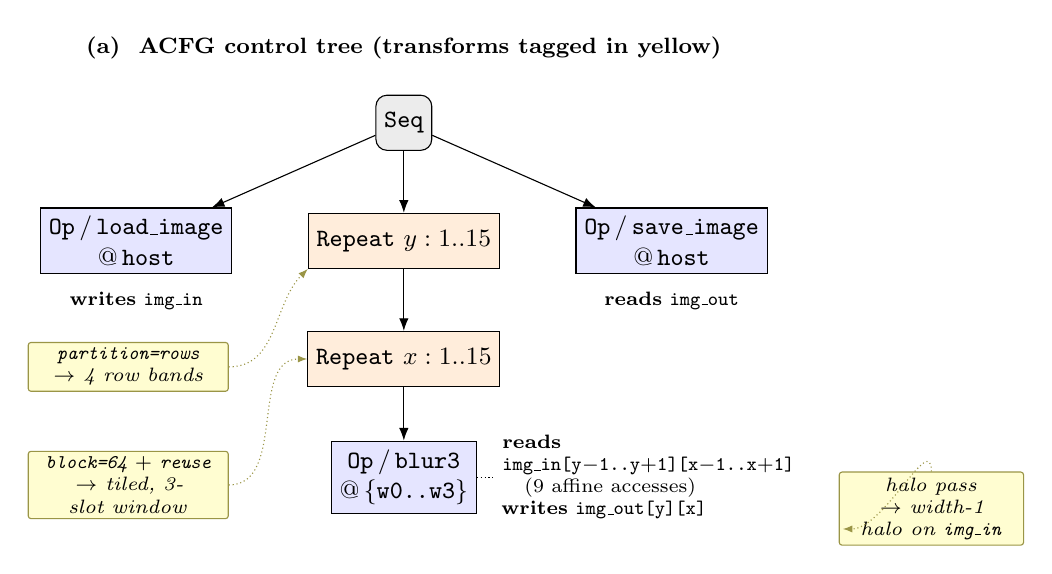
\begin{tikzpicture}[
      font=\small,
      seq/.style={draw, rounded corners, fill=gray!15, minimum height=7mm,
                  inner sep=3pt, align=center},
      op/.style={draw, fill=blue!10, minimum height=7mm, inner sep=3pt, align=center},
      rep/.style={draw, fill=orange!14, minimum height=7mm, inner sep=3pt, align=center},
      tree/.style={-{Latex[length=1.6mm]}},
      tag/.style={font=\scriptsize\itshape, fill=yellow!18, draw=yellow!55!black,
                  rounded corners=1pt, inner sep=2pt, align=center},
      lead/.style={densely dotted, yellow!55!black, -{Latex[length=1.2mm]}},
    ]
    \node[seq] (seq) at (0,0) {\texttt{Seq}};
    \node[op]  (load) at (-3.4,-1.5) {\texttt{Op}\,/\,\texttt{load\_image}\\@\,\texttt{host}};
    \node[rep] (ry)   at (0,-1.5)    {\texttt{Repeat} $y:1..15$};
    \node[op]  (save) at (3.4,-1.5)  {\texttt{Op}\,/\,\texttt{save\_image}\\@\,\texttt{host}};
    \node[rep] (rx)   at (0,-3.0)    {\texttt{Repeat} $x:1..15$};
    \node[op]  (blur) at (0,-4.5)    {\texttt{Op}\,/\,\texttt{blur3}\\@\,$\{$\texttt{w0..w3}$\}$};
    \draw[tree] (seq) -- (load);
    \draw[tree] (seq) -- (ry);
    \draw[tree] (seq) -- (save);
    \draw[tree] (ry) -- (rx);
    \draw[tree] (rx) -- (blur);

    % dataflow records (the affine read/write sets) to the right of each op
    \node[align=left, font=\scriptsize, right=2mm of blur, text width=42mm] (df) {%
      \textbf{reads} \texttt{img\_in[y$-$1..y$+$1][x$-$1..x$+$1]}\\
      \quad (9 affine accesses)\\
      \textbf{writes} \texttt{img\_out[y][x]}};
    \draw[densely dotted] (blur) -- (df);
    \node[font=\scriptsize, below=1mm of load] (dfl) {\textbf{writes} \texttt{img\_in}};
    \node[font=\scriptsize, below=1mm of save] (dfs) {\textbf{reads} \texttt{img\_out}};

    % schedule-transform tags, stacked in the empty lower-left, with leaders
    \node[tag, text width=24mm] (tpar) at (-3.5,-3.1)
      {\texttt{partition=rows}\\$\rightarrow$ 4 row bands};
    \node[tag, text width=24mm] (tblk) at (-3.5,-4.6)
      {\texttt{block=64} $+$ \texttt{reuse}\\$\rightarrow$ tiled, 3-slot window};
    \node[tag, text width=22mm] (thalo) at (6.7,-4.9)
      {halo pass\\$\rightarrow$ width-1 halo on \texttt{img\_in}};
    \draw[lead] (tpar.east) to[out=0,in=-135] (ry.south west);
    \draw[lead] (tblk.east) to[out=0,in=180] (rx.west);
    \draw[lead] (thalo.north) to[out=90,in=0] (df.south east);

    \node[font=\footnotesize\bfseries] at (0,0.95)
      {(a)\ \ ACFG control tree (transforms tagged in yellow)};
  \end{tikzpicture}

  \vspace{3mm}

  {\footnotesize\bfseries (b)\ \ dataflow DAG (the \emph{what}, before any decomposition)}\par
  \vspace{1.5mm}

  % ===== Panel (b): the dataflow DAG (resized to fit the text width) =====
  \resizebox{\textwidth}{!}{%
  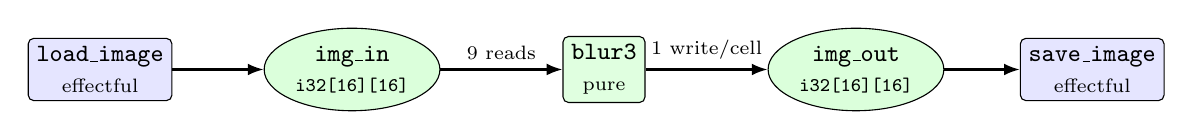
\begin{tikzpicture}[
      font=\small,
      data/.style={draw, ellipse, fill=green!14, inner sep=2pt, align=center},
      kern/.style={draw, rounded corners=2pt, inner sep=3pt, align=center},
      flow/.style={-{Latex[length=2mm]}, thick},
    ]
    \node[kern, fill=blue!10] (k1) at (0,0) {\texttt{load\_image}\\\scriptsize effectful};
    \node[data] (d1) at (3.2,0) {\texttt{img\_in}\\\scriptsize\texttt{i32[16][16]}};
    \node[kern, fill=green!12] (k2) at (6.4,0) {\texttt{blur3}\\\scriptsize pure};
    \node[data] (d2) at (9.6,0) {\texttt{img\_out}\\\scriptsize\texttt{i32[16][16]}};
    \node[kern, fill=blue!10] (k3) at (12.6,0) {\texttt{save\_image}\\\scriptsize effectful};
    \draw[flow] (k1) -- (d1);
    \draw[flow] (d1) -- node[above, font=\scriptsize]{9 reads} (k2);
    \draw[flow] (k2) -- node[above, font=\scriptsize]{1 write/cell} (d2);
    \draw[flow] (d2) -- (k3);
  \end{tikzpicture}}

  \caption[The stencil's ACFG and dataflow DAG]{The application control-flow
    graph the compiler builds for the stencil. \textbf{(a)} The control tree: a
    \texttt{Seq} of an effectful load, a doubly-nested \texttt{Repeat} firing the
    pure \texttt{blur3}, and an effectful save (\texttt{@} denotes placement, so
    \texttt{@\{w0..w3\}} means the operation runs on all four compute workers).
    Each operation carries a dataflow record naming the arrays it reads and
    writes as affine index expressions (dotted). The schedule's transforms (yellow) rewrite or annotate specific
    nodes: \texttt{partition=rows} cuts the $y$ repeat into four bands,
    \texttt{block=64} with \texttt{reuse} tiles the $x$ repeat and adds a
    three-slot delay line, and halo inference records a width-one halo on
    \texttt{img\_in}. \textbf{(b)} The same body as a dataflow DAG --- still the
    \emph{what}, with no worker, transfer, or buffer in sight. Loop ranges are
    half-open ($1..15$ denotes $1,\dots,14$).}
  \label{fig:wt-acfg}
\end{figure}


The schedule's transforms are then applied to this tree, in the fixed order the
pipeline defines, each pass either rewriting the tree or annotating it. Throughout,
loop and band ranges are written half-open: $a..b$ denotes the integers
$a, a{+}1, \dots, b{-}1$.

\begin{itemize}
  \item \textbf{Tiling.} The \texttt{block=64} directive on \texttt{x} strip-mines
        the inner loop into a tile loop over an outer tile index and an intra-tile
        loop. The interior \texttt{x} range is $1..15$, of length 14; since the
        block size 64 exceeds it, there is a single tile here. The structure is
        nonetheless materialised, so the same code path handles the partial-tile
        case that arises when the block does not divide the range.
  \item \textbf{Partitioning.} The \texttt{partition=rows} directive on \texttt{y}
        is consumed by the row-band pass, which overrides each compute worker's
        \texttt{y} range with its band. The outer range $1..15$ likewise has length
        14, which does not divide evenly by four; the compiler distributes the
        remainder with a floor-with-spillover policy, handing
        $\lceil 14/4 \rceil = 4$ rows to the first two workers and
        $\lfloor 14/4 \rfloor = 3$ to the last two, giving the contiguous bands
        $1..5$, $5..9$, $9..12$, $12..15$ (\cref{fig:wt-bands}). The partition passes for
        per-worker ranges, row bands, and two-dimensional grids are mutually
        exclusive alternatives selected by the directive; here only the row-band
        pass fires.
  \item \textbf{Halo inference.} The halo pass reads \texttt{blur3}'s access
        pattern and finds that each output row $y$ reads input rows $y-1$, $y$, and
        $y+1$ (and analogously $x-1, x, x+1$): offsets of $-1$, $0$, $+1$ in both
        dimensions, recognised because each index is affine in the loop variable.
        It records a halo of width one on \texttt{img\_in} along the partitioned
        \texttt{y} axis. This is the fact that makes a row-band partition correct:
        a worker computing rows $1..5$ needs input rows $0..6$ --- its band plus one
        halo row above and below.
  \item \textbf{Reuse inference.} The \texttt{reuse} directive on \texttt{x} is
        discharged by the reuse pass, which recognises that as \texttt{x} advances
        by one the three-wide window of \texttt{img\_in} reads shifts by one, so two
        of every three reads can be carried over. It annotates the loop with a
        three-slot circular delay line per input row. This is the optimisation
        earlier iterations of the system could not express; here it falls out of a
        one-word directive and the access pattern.
\end{itemize}

% fig:wt-bands --- the row-band partition with the floor-with-spillover remainder
% and the width-1 halo. Faithful to sec:wt-acfg / sec:wt-inject of
% chapters/07b-compilation-walkthrough.tex:
%   interior y range 1..15 (length 14), partitioned 4/4/3/3 across w0..w3:
%     w0 = 1..5,  w1 = 5..9,  w2 = 9..12,  w3 = 12..15   (output bands, half-open)
%   halo width 1 on img_in along y => each worker receives band +- 1 row:
%     w0 input 0..6,  w1 input 4..10,  w2 input 8..13,  w3 input 11..16
%   rows 0 and 15 are the never-written border (interior is 1..15).
\begin{figure}[tbp]
  \centering
  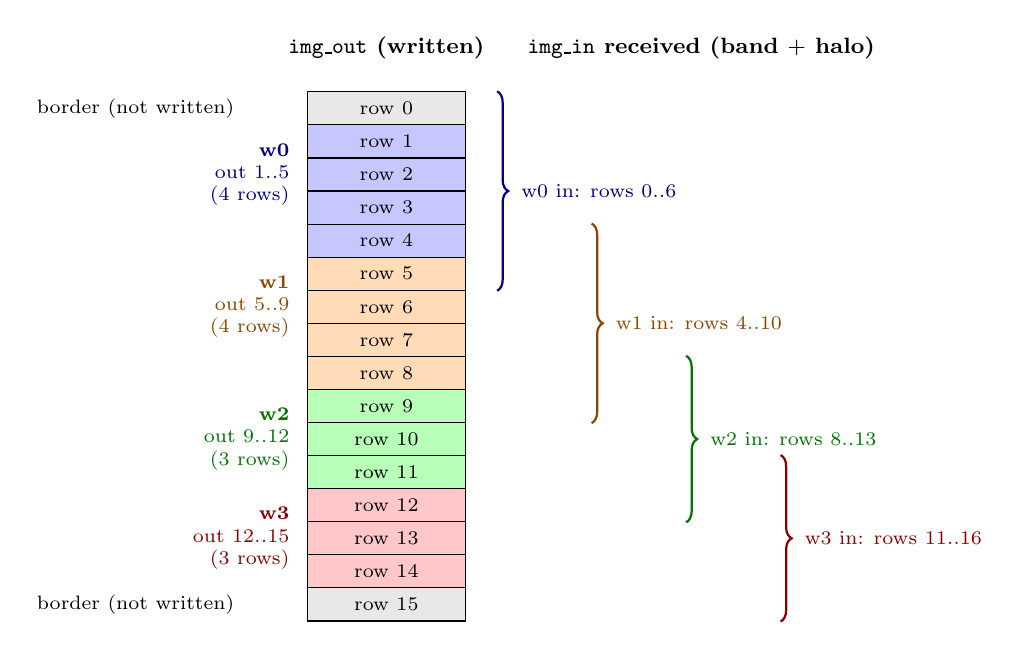
\begin{tikzpicture}[
      font=\small,
      cell/.style={draw, minimum width=20mm, minimum height=4.2mm,
                   inner sep=0pt, anchor=north},
      brace/.style={decorate, decoration={brace, amplitude=4pt}, thick},
    ]
    % geometry: row r drawn at y = -r*0.42 cm (row 0 at top).
    \def\rh{0.42}
    \foreach \r in {0,...,15} {
      \pgfmathsetmacro\yy{-\r*\rh}
      % default border colour
      \def\fillcol{gray!18}
      \ifnum\r>0 \ifnum\r<5 \def\fillcol{blue!22}\fi\fi      % w0 band rows 1..4
      \ifnum\r>4 \ifnum\r<9 \def\fillcol{orange!28}\fi\fi    % w1 band rows 5..8
      \ifnum\r>8 \ifnum\r<12 \def\fillcol{green!28}\fi\fi    % w2 band rows 9..11
      \ifnum\r>11 \ifnum\r<15 \def\fillcol{red!22}\fi\fi     % w3 band rows 12..14
      \node[cell, fill=\fillcol] (row\r) at (0,\yy) {\scriptsize row \r};
    }
    % left header
    \node[font=\footnotesize\bfseries, align=center] at (0,0.55)
      {\texttt{img\_out} (written)};
    \node[font=\scriptsize, left=8mm of row0, anchor=east] {border (not written)};
    \node[font=\scriptsize, left=8mm of row15, anchor=east] {border (not written)};

    % band labels (output) on the left
    \node[font=\scriptsize, blue!50!black, left=1mm of row2.west, anchor=east, align=right]
      {\textbf{w0}\\out $1..5$\\(4 rows)};
    \node[font=\scriptsize, orange!55!black, left=1mm of row6.west, anchor=east, align=right]
      {\textbf{w1}\\out $5..9$\\(4 rows)};
    \node[font=\scriptsize, green!45!black, left=1mm of row10.west, anchor=east, align=right]
      {\textbf{w2}\\out $9..12$\\(3 rows)};
    \node[font=\scriptsize, red!55!black, left=1mm of row13.west, anchor=east, align=right]
      {\textbf{w3}\\out $12..15$\\(3 rows)};

    % halo-input ranges as braces on the right.  Each worker receives its band
    % +-1 halo row.  Braces drawn at increasing x to show the overlaps (halo).
    % w0 input rows 0..5 (range 0..6)
    \draw[brace, blue!50!black] ([xshift=4mm]row0.north east) -- ([xshift=4mm]row5.south east)
      node[midway, right=5pt, font=\scriptsize, align=left, blue!50!black]
      {w0 in: rows $0..6$};
    % w1 input rows 4..9 (range 4..10)
    \draw[brace, orange!55!black] ([xshift=16mm]row4.north east) -- ([xshift=16mm]row9.south east)
      node[midway, right=5pt, font=\scriptsize, align=left, orange!55!black]
      {w1 in: rows $4..10$};
    % w2 input rows 8..12 (range 8..13)
    \draw[brace, green!45!black] ([xshift=28mm]row8.north east) -- ([xshift=28mm]row12.south east)
      node[midway, right=5pt, font=\scriptsize, align=left, green!45!black]
      {w2 in: rows $8..13$};
    % w3 input rows 11..15 (range 11..16)
    \draw[brace, red!55!black] ([xshift=40mm]row11.north east) -- ([xshift=40mm]row15.south east)
      node[midway, right=5pt, font=\scriptsize, align=left, red!55!black]
      {w3 in: rows $11..16$};

    \node[font=\footnotesize\bfseries, align=center] at (4.0,0.55)
      {\texttt{img\_in} received (band $+$ halo)};
  \end{tikzpicture}
  \caption[Row-band partition and halo of the stencil]{The row-band partition of
    the stencil's outer loop. The interior range $1..15$ (rows $1$ through $14$;
    rows $0$ and $15$ are the never-written border) has length $14$, which does
    not divide evenly by four. The floor-with-spillover policy hands
    $\lceil 14/4\rceil = 4$ rows to \texttt{w0} and \texttt{w1} and
    $\lfloor 14/4\rfloor = 3$ to \texttt{w2} and \texttt{w3}, giving the
    contiguous output bands $1..5$, $5..9$, $9..12$, $12..15$ (left). Halo
    inference adds one row on each side along $y$, so each worker receives a
    \emph{larger} slice of \texttt{img\_in} (right braces): \texttt{w0} computing
    $1..5$ receives input rows $0..6$, \texttt{w1} computing $5..9$ receives
    $4..10$, and so on. The brace overlaps are the shared halo rows. All ranges
    are half-open.}
  \label{fig:wt-bands}
\end{figure}


After these passes the ACFG is no longer a faithful echo of the source loop nest:
it encodes four per-worker bands, a tiled and reuse-windowed inner loop, and the
knowledge that \texttt{img\_in} carries a one-row halo --- yet still contains no
transfers or synchronisations. Those are injected next.

\section{Injecting synchronisation and transfers}\label{sec:wt-inject}

Two final middle-end passes turn the decomposition implied by the ACFG into
explicit coordination: the synchronisation pass and the transfer pass
(\cref{sec:arch-transfer}). The synchronisation pass inserts the barriers that
bracket the distributed phase: one before the compute workers begin, after the host
has the input ready, and one after they finish, before the host collects the
output. Each barrier names its participants --- here all five workers --- and is
given a stable \emph{sync tag}, a compile-time identifier shared by every
participant of that barrier (\cref{sec:arch-petri}), so the projection can match the
same barrier across workers without a global walk.

The transfer pass then consumes the producer/consumer facts from linking and the
halo width from inference, and synthesises matched send/receive pairs. For
\texttt{img\_in} it emits, for each compute worker, a transfer from the host
carrying that worker's band \emph{plus its halo rows}: worker \texttt{w0}, which
computes rows $1..5$, receives input rows $0..6$; worker \texttt{w1}, computing
$5..9$, receives rows $4..10$; and so on. These transfers carry the schedule's
\texttt{img\_in} policy --- asynchronous, two-deep buffer, event notification. For
\texttt{img\_out} it emits, for each compute worker, a transfer back to the host
carrying just that worker's band of results, under the synchronous policy (a
single-deep, blocking channel: the host receives each band before the worker could
send another). The result is the fully elaborated ACFG: decomposition, halos, synchronisation, and IO
semantics all explicit, and still not one line of backend-specific code.

\section{The Petri net and the soundness gate}\label{sec:wt-net}

The elaborated ACFG is now lowered to a Petri net and checked
(\cref{sec:arch-gate,fig:wt-net}). In a Petri net, \emph{places} hold tokens up to a
capacity and \emph{transitions} fire by consuming tokens from their input places and
producing tokens in their output places. Here places model the things that hold
state --- each array region a worker owns, each transfer channel, and each barrier
--- and transitions model the things that happen: the host's \texttt{load\_image} firing,
the four \texttt{img\_in} sends and their matching receives, each worker's
\texttt{blur3} firings, the two barriers, the four \texttt{img\_out} sends and
receives, and the host's \texttt{save\_image} firing. A channel place has a finite
capacity drawn from the transfer's buffer policy --- two for the asynchronous
\texttt{img\_in} channels, one for the synchronous \texttt{img\_out} channels.

The gate runs its three checks in a fixed order (\cref{sec:arch-gate}). It first
confirms \emph{conflict-freedom}: no place offers a token to two competing
consumers. This is the load-bearing precondition. For the restricted net class this
language produces --- which by construction has no data-dependent token routing ---
conflict-freedom removes the only remaining source of choice, so every firing order
is a permutation of one partial order and reaches the same states; that is what
makes a single replayed order representative of all of them. The argument is
specific to this class and is not a general Petri-net property. On that basis the
gate derives one deterministic firing order and replays it, checking
\emph{boundedness} --- no channel place ever exceeds the capacity its buffer policy
sets --- and \emph{deadlock-freedom} --- no required transition is left permanently
un-fireable, whether because an input place never receives its token or because a
bounded output place stays full in a cyclic wait. For the stencil the net passes:
the two-deep input buffers never overflow, because the host pushes exactly one band
into each per-worker channel before reaching the barrier, well within the two-deep
capacity; and the barriers admit a completing order. Had the schedule
asked for a single-deep buffer where two were needed, or arranged a cyclic wait,
the gate would have rejected the program here, at compile time, naming the
offending place or transition --- not produced code that hangs. This check runs on
this program, as on every program, before any code is emitted.

% fig:wt-net --- the Petri net the elaborated ACFG lowers to, and the soundness
% gate. Faithful to sec:wt-net of chapters/07b-compilation-walkthrough.tex:
%   places  = array regions a worker owns, transfer channels, barriers;
%   transitions = host load_image, 4 img_in sends + 4 matching receives,
%                 each worker's blur3 firings, the two barriers,
%                 4 img_out sends + receives, host save_image.
%   channel capacities: 2 for the async img_in channels, 1 for the sync img_out.
% The four compute workers are a 4-fold-symmetric column; drawn once inside a
% plate ("x4") for legibility, with the host spine across the top. The two
% barriers are 5-way (host + w0..w3).
\begin{figure}[tbp]
  \centering
  \resizebox{\textwidth}{!}{%
  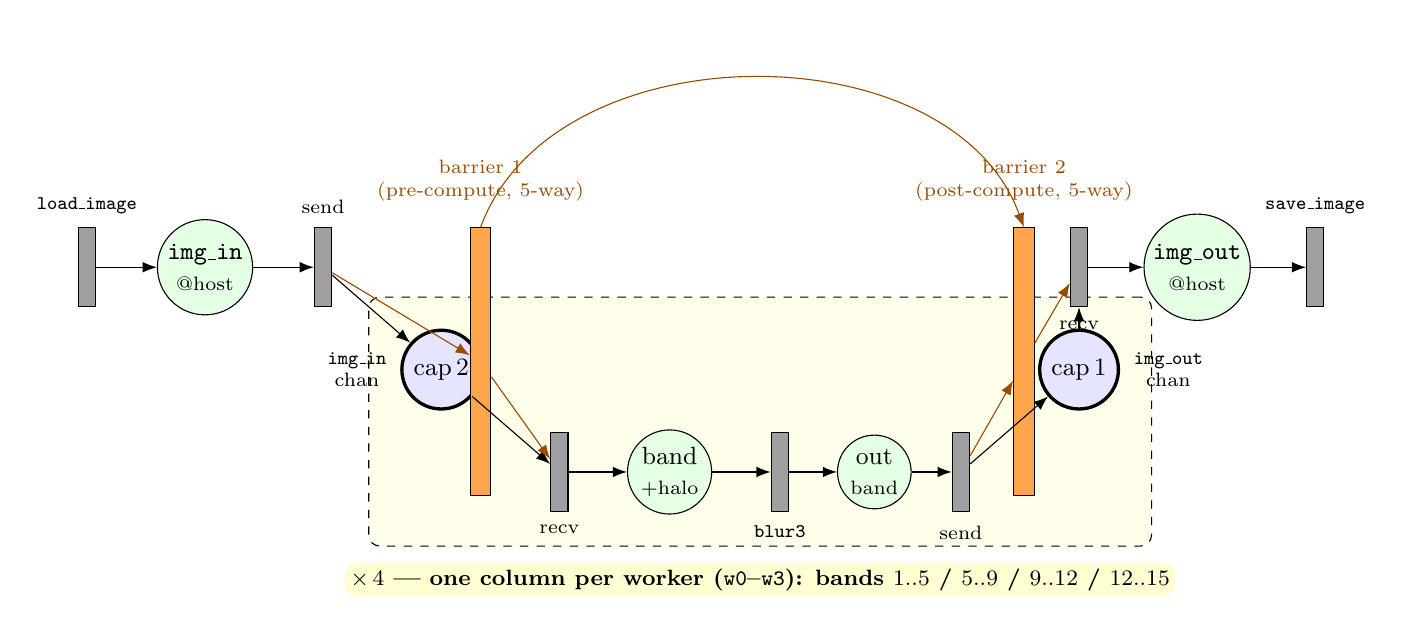
\begin{tikzpicture}[
      font=\small,
      place/.style={draw, circle, minimum size=9mm, inner sep=1pt, align=center,
                    fill=green!10},
      chan/.style={draw, circle, minimum size=10mm, inner sep=1pt, align=center,
                   fill=blue!10, very thick},
      tr/.style={draw, fill=gray!75, minimum width=2.2mm, minimum height=10mm,
                 inner sep=0pt},
      bar/.style={draw, fill=orange!70, minimum width=2.6mm, minimum height=34mm,
                  inner sep=0pt},
      a/.style={-{Latex[length=1.8mm]}},
      lbl/.style={font=\scriptsize, align=center},
    ]
    % ---- host spine (y = 2.6) ----
    \def\hy{2.6}
    \node[tr] (tload) at (0,\hy) {};   \node[lbl, above=0.5mm of tload] {\texttt{load\_image}};
    \node[place] (pin) at (1.5,\hy) {\texttt{img\_in}\\\scriptsize @host};
    \node[tr] (tsend) at (3.0,\hy) {}; \node[lbl, above=0.5mm of tsend] {send};
    \node[tr] (trout) at (12.6,\hy) {};\node[lbl, below=0.5mm of trout] {recv};
    \node[place] (pout) at (14.1,\hy) {\texttt{img\_out}\\\scriptsize @host};
    \node[tr] (tsave) at (15.6,\hy) {};\node[lbl, above=0.5mm of tsave] {\texttt{save\_image}};

    % ---- a single worker column (y = 0), enclosed by a plate ----
    \node[chan] (cin) at (4.5,1.3) {cap\,2};
    \node[lbl, left=0.5mm of cin] {\texttt{img\_in}\\chan};
    \node[tr] (trin) at (6.0,0) {};   \node[lbl, below=0.5mm of trin] {recv};
    \node[place] (pband) at (7.4,0) {band\\\scriptsize $+$halo};
    \node[tr] (tblur) at (8.8,0) {}; \node[lbl, below=0.5mm of tblur] {\texttt{blur3}};
    \node[place] (pob) at (10.0,0) {out\\\scriptsize band};
    \node[tr] (tso) at (11.1,0) {};  \node[lbl, below=0.5mm of tso] {send};
    \node[chan] (cout) at (12.6,1.3) {cap\,1};
    \node[lbl, right=0.5mm of cout] {\texttt{img\_out}\\chan};

    % plate around the worker column
    \begin{scope}[on background layer]
      \node[draw, dashed, rounded corners, fill=yellow!8, inner sep=4mm,
            fit=(cin)(trin)(pband)(tblur)(pob)(tso)(cout),
            label={[font=\footnotesize\bfseries, fill=yellow!18, rounded corners,
                    inner sep=2pt, yshift=-2mm]below:$\times\,4$ --- one column per
                    worker (\texttt{w0}--\texttt{w3}): bands $1..5$ / $5..9$ /
                    $9..12$ / $12..15$}]
            (plate) {};
    \end{scope}

    % ---- the two 5-way barriers ----
    \node[bar] (b1) at (5.0,1.4) {};
    \node[lbl, orange!60!black] at (5.0,3.7) {barrier 1\\\scriptsize (pre-compute, 5-way)};
    \node[bar] (b2) at (11.9,1.4) {};
    \node[lbl, orange!60!black] at (11.9,3.7) {barrier 2\\\scriptsize (post-compute, 5-way)};

    % ---- arcs ----
    \draw[a] (tload) -- (pin);
    \draw[a] (pin) -- (tsend);
    \draw[a] (tsend) -- (cin);            % host pushes into the img_in channel
    \draw[a] (cin) -- (trin);             % worker receives
    \draw[a] (trin) -- (pband);
    \draw[a] (pband) -- (tblur);
    \draw[a] (tblur) -- (pob);
    \draw[a] (pob) -- (tso);
    \draw[a] (tso) -- (cout);             % worker pushes into img_out channel
    \draw[a] (cout) -- (trout);           % host receives
    \draw[a] (trout) -- (pout);
    \draw[a] (pout) -- (tsave);
    % barrier synchronisation arcs (host + worker both meet each barrier)
    \draw[a, orange!60!black] (tsend) -- (b1);
    \draw[a, orange!60!black] (b1) -- (trin);
    \draw[a, orange!60!black] (tso) -- (b2);
    \draw[a, orange!60!black] (b2) -- (trout);
    % host participates in BOTH barriers: it passes barrier 1, idles, then meets
    % barrier 2 (the back-to-back "barrier; barrier" in the host's event list).
    \draw[a, orange!60!black] (b1.north) to[out=70,in=110] (b2.north);
  \end{tikzpicture}}
  \caption[The stencil's Petri net and soundness gate]{The Petri net the
    elaborated ACFG lowers to. \emph{Places} (circles) model state --- the array
    regions a worker owns and the transfer channels --- and \emph{transitions}
    (bars) model events: the host's \texttt{load\_image}, the four
    \texttt{img\_in} sends and matching receives, each worker's \texttt{blur3}
    firings, the four \texttt{img\_out} sends and receives, and the host's
    \texttt{save\_image}. The four compute workers form a 4-fold-symmetric
    column, drawn once inside the dashed plate. Channel places (marked
    ``cap'') carry the capacity their buffer policy sets: \textbf{2} for the
    asynchronous \texttt{img\_in} channels, \textbf{1} for the synchronous
    \texttt{img\_out} channels. The two orange bars are the 5-way (host $+$
    \texttt{w0}--\texttt{w3}) pre- and post-compute barriers; the orange arcs
    are their barrier-place arcs (no participant proceeds until all five have
    arrived), and the arc arching over the top is the host idling from the
    first barrier to the second. The gate checks, in order, conflict-freedom
    (no place offers a token to two competing consumers), then --- on one
    replayed firing order --- boundedness (no \texttt{img\_in} channel ever
    exceeds 2) and deadlock-freedom, before any code is emitted.}
  \label{fig:wt-net}
\end{figure}


\section{Projection to per-worker event lists}\label{sec:wt-events}

The last middle-end step projects the elaborated ACFG into one totally-ordered
event list per worker (\cref{sec:arch-projection,fig:wt-events}). The walk is
deterministic, so the lists are reproducible byte-for-byte across compilations. The
events are drawn from a small fixed vocabulary --- fire a kernel, push a data region
to a worker, wait for a region from a worker, participate in a barrier, and loop ---
and they are the \emph{sole} interface to the backend: everything the decomposition
decided is encoded in them, and nothing else crosses the line.

For the stencil the host's list reads: fire \texttt{load\_image}; push
\texttt{img\_in} to \texttt{w0}, \texttt{w1}, \texttt{w2}, \texttt{w3}; barrier;
barrier; wait for \texttt{img\_out} from \texttt{w0}, \texttt{w1}, \texttt{w2},
\texttt{w3}; fire \texttt{save\_image}. The host stages all four input bands into
the buffered channels, then the two barriers bracket the phase during which it has
nothing to do, then it collects the four output bands. The two barriers are the
same pre- and post-compute synchronisations of \cref{sec:wt-inject}: the first
releases the workers once every input band has been pushed, the second waits until
every worker has finished and pushed its output. Each compute worker's list is the
mirror image. Worker \texttt{w0}'s reads: barrier; wait for \texttt{img\_in} from
the host; a loop over its band rows $1..5$, whose body is the tiled, reuse-windowed
inner loop firing \texttt{blur3}; push \texttt{img\_out} to the host; barrier. The
loop event carries the iteration structure rather than an unrolled body, so a
backend emits a loop construct rather than one replicated body per iteration,
keeping generated code compact regardless of trip count.

% fig:wt-events --- the per-worker event lists as a swimlane timeline.
% Faithful to sec:wt-events of chapters/07b-compilation-walkthrough.tex:
%   host : fire load_image; push img_in to w0,w1,w2,w3; barrier; barrier;
%          wait img_out from w0,w1,w2,w3; fire save_image.
%   w_i  : barrier; wait img_in from host; loop over band { tiled+reuse blur3 };
%          push img_out to host; barrier.
% Time flows downward. The two barriers are horizontal 5-way sync lines; the host
% idles (empty lane) between them while the workers compute -- which is exactly
% the host's back-to-back "barrier; barrier" in its list.
\begin{figure}[tbp]
  \centering
  \resizebox{\textwidth}{!}{%
  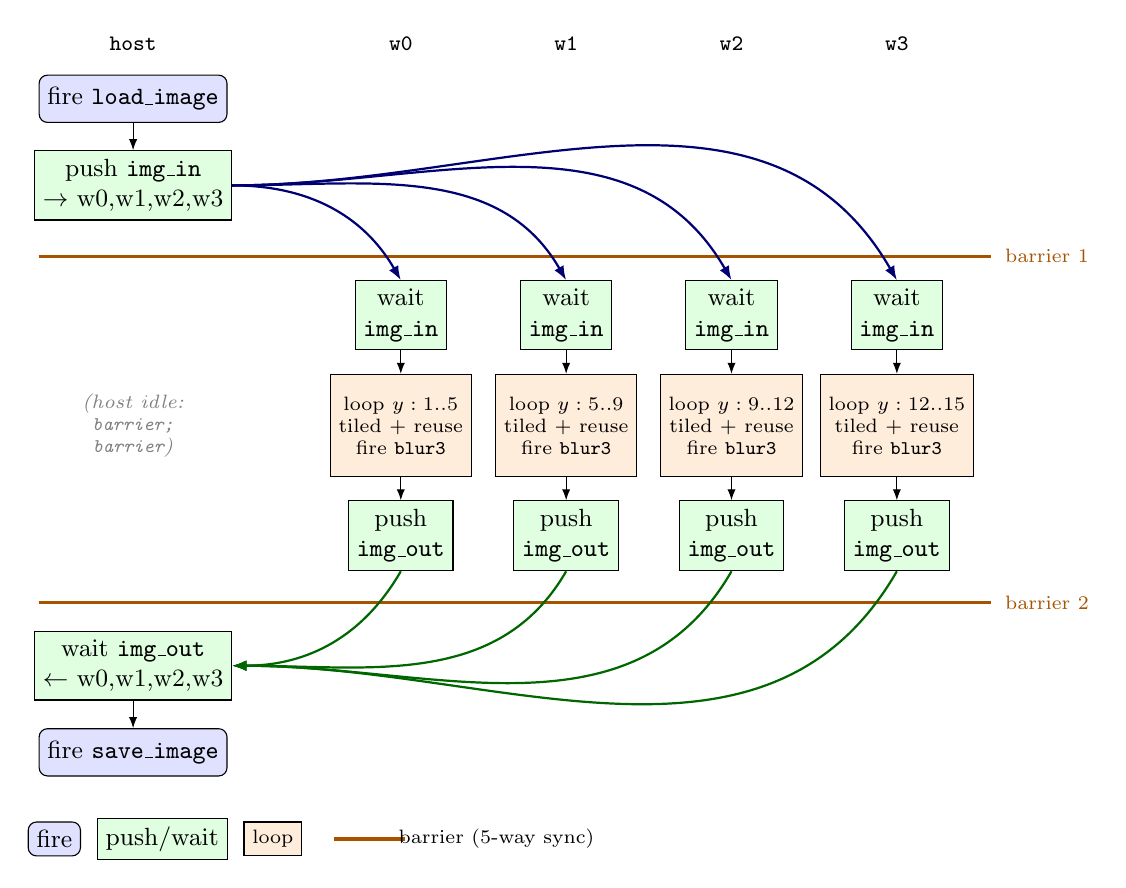
\begin{tikzpicture}[
      font=\small,
      fire/.style={draw, rounded corners=3pt, fill=blue!12, minimum height=6mm,
                   inner sep=3pt, align=center},
      io/.style={draw, fill=green!12, minimum height=6mm, inner sep=3pt, align=center},
      loop/.style={draw, fill=orange!14, minimum height=13mm, inner sep=3pt,
                   align=center, font=\scriptsize},
      bar/.style={very thick, orange!65!black},
      lane/.style={font=\footnotesize\bfseries},
      push/.style={-{Latex[length=1.8mm]}, blue!45!black, thick},
      ret/.style={-{Latex[length=1.8mm]}, green!40!black, thick},
    ]
    % lane x positions
    \def\xh{0} \def\xa{3.4} \def\xb{5.5} \def\xc{7.6} \def\xd{9.7}
    % lane headers
    \node[lane] at (\xh,0.7) {\texttt{host}};
    \node[lane] at (\xa,0.7) {\texttt{w0}};
    \node[lane] at (\xb,0.7) {\texttt{w1}};
    \node[lane] at (\xc,0.7) {\texttt{w2}};
    \node[lane] at (\xd,0.7) {\texttt{w3}};

    % --- host lane above barrier 1 ---
    \node[fire] (hload) at (\xh,0)   {fire \texttt{load\_image}};
    \node[io]   (hpush) at (\xh,-1.1){push \texttt{img\_in}\\$\rightarrow$ w0,w1,w2,w3};

    % --- barrier 1 (5-way) ---
    \def\byone{-2.0}
    \draw[bar] (-1.2,\byone) -- (10.9,\byone);
    \node[font=\scriptsize, anchor=west, orange!65!black] at (10.95,\byone) {barrier 1};

    % --- worker lanes between the barriers ---
    \foreach \x/\name/\band in {\xa/w0/{1..5}, \xb/w1/{5..9}, \xc/w2/{9..12}, \xd/w3/{12..15}} {
      \node[io]   (\name wait) at (\x,-2.75) {wait\\\texttt{img\_in}};
      \node[loop] (\name loop) at (\x,-4.15) {loop $y:\band$\\\scriptsize tiled $+$ reuse\\\scriptsize fire \texttt{blur3}};
      \node[io]   (\name out)  at (\x,-5.55) {push\\\texttt{img\_out}};
    }
    % host idles between the two barriers (empty lane) -- its list is "barrier; barrier"
    \node[font=\scriptsize\itshape, gray, align=center] at (\xh,-4.15)
      {(host idle:\\\texttt{barrier;}\\\texttt{barrier})};

    % --- barrier 2 (5-way) ---
    \def\bytwo{-6.4}
    \draw[bar] (-1.2,\bytwo) -- (10.9,\bytwo);
    \node[font=\scriptsize, anchor=west, orange!65!black] at (10.95,\bytwo) {barrier 2};

    % --- host lane below barrier 2 ---
    \node[io]   (hwait) at (\xh,-7.2) {wait \texttt{img\_out}\\$\leftarrow$ w0,w1,w2,w3};
    \node[fire] (hsave) at (\xh,-8.3) {fire \texttt{save\_image}};

    % --- intra-lane order edges (host) ---
    \draw[-{Latex[length=1.4mm]}] (hload) -- (hpush);
    \draw[-{Latex[length=1.4mm]}] (hwait) -- (hsave);
    % --- intra-lane order edges (workers) ---
    \foreach \name in {w0,w1,w2,w3} {
      \draw[-{Latex[length=1.4mm]}] (\name wait) -- (\name loop);
      \draw[-{Latex[length=1.4mm]}] (\name loop) -- (\name out);
    }
    % --- cross-lane transfers: img_in pushes (host -> workers) ---
    \foreach \name in {w0,w1,w2,w3} {
      \draw[push] (hpush.east) to[out=0,in=120] (\name wait.north);
    }
    % --- cross-lane transfers: img_out returns (workers -> host) ---
    \foreach \name in {w0,w1,w2,w3} {
      \draw[ret] (\name out.south) to[out=-120,in=0] (hwait.east);
    }

    % --- legend ---
    \begin{scope}[shift={(-1.0,-9.4)}]
      \node[fire, minimum height=4mm] (lf) at (0,0) {fire};
      \node[io, minimum height=4mm, right=2mm of lf] (li) {push/wait};
      \node[loop, minimum height=4mm, right=2mm of li] (ll) {loop};
      \draw[bar] ([xshift=4mm]ll.east) -- ++(0.9,0);
      \node[font=\scriptsize, right=1mm of ll, xshift=10mm] {barrier (5-way sync)};
    \end{scope}
  \end{tikzpicture}}
  \caption[Per-worker event lists of the stencil]{The per-worker event lists, the
    sole interface between the middle end and any backend, as a swimlane
    timeline (time flows down). The host fires \texttt{load\_image}, pushes one
    \texttt{img\_in} band into each worker's buffered channel, meets both
    barriers, collects the four \texttt{img\_out} bands, and fires
    \texttt{save\_image}. Each worker meets barrier 1, waits for its
    \texttt{img\_in} band, runs the tiled, reuse-windowed \texttt{blur3} loop over
    its row band, pushes its \texttt{img\_out} band back, and meets barrier 2. The
    two horizontal bars are the 5-way pre- and post-compute barriers; between them
    the host lane is empty --- exactly the back-to-back \texttt{barrier; barrier}
    in the host's list --- while the workers compute. Blue arrows are
    \texttt{img\_in} transfers (host to worker), green arrows are
    \texttt{img\_out} transfers (worker to host); the \texttt{img\_in} pushes
    cross barrier 1 because the channels are buffered (depth 2). The loop event
    carries the iteration structure, not an unrolled body.}
  \label{fig:wt-events}
\end{figure}


These event lists are the output of the middle end and the input to every backend.
The same host-and-four-workers lists just described are what the next sections lower
to shared-memory threads, to MPI ranks, and to bare-metal microcontrollers --- the
same events, three very different renderings.

\section{One event list, three renderings}\label{sec:wt-lowering}

A backend consumes the per-worker event lists and nothing else
(\cref{sec:arch-codegen}). It renders each event into code for one combination of
runtime and transport, and the central observation of this chapter is visible only
once that rendering is laid side by side across backends: the events that compute
--- fire a kernel, loop --- go through a \emph{shared} renderer, while only the events
that communicate --- push, wait, barrier --- are rendered per-backend
(\cref{fig:wt-lowering}). This is the middle-end/presentation boundary
(\cref{sec:arch-boundaries}) --- the line separating the shared, backend-independent
lowering from the per-backend rendering of transport --- made mechanical: there is one
emitter for the inside of a worker and a small per-backend emitter for the seams
between workers.

The consequence is literal, not approximate. Emitting the stencil's distributed event
lists to the shared-memory \texttt{pthreads-async} backend and to the
distributed-memory \texttt{mpi-nonblocking} backend produces, for each compute
worker, \emph{byte-for-byte the same compute body} --- the same tiled, reuse-windowed
loop, the same nine-argument \texttt{blur3} call, the same circular-buffer index
arithmetic, down to the character (the transport sections of the two files, of
course, differ). The two generated programs diverge only where a worker sends or
receives a band or meets a barrier. The sections below show each of the three
renderings of the same event lists from \cref{sec:wt-events} --- two of them, the
hosted backends, running that exact distributed schedule, the third running a
synchronous variant its transport requires --- and the last explains why all three
agree to the byte.

\section{Shared memory: the pthreads rendering}\label{sec:wt-pthreads}

The \texttt{pthreads-async} backend maps each worker to an operating-system thread
and each transfer channel to a bounded ring buffer shared between two threads
(\cref{sec:be-tier1}). The host's \texttt{main} allocates one ring per transfer ---
four for the \texttt{img\_in} sends, each a two-slot ring matching the schedule's
\texttt{buffer=2}, and four single-slot rings for the synchronous \texttt{img\_out}
returns --- and two five-party barriers, then spawns the four compute-worker threads
and runs the host's own event list inline.

Each event renders to a shared-memory primitive. A \emph{push} becomes a
\texttt{ring.push(payload)} into the destination worker's channel; a \emph{wait}
becomes a \texttt{ring.wait()} followed by a copy of the received band into the
worker's local array; a \emph{barrier} becomes a \texttt{barrier.wait()} on the
shared five-party barrier; and a \emph{fire} becomes a direct call to the kernel.
The ring is a condition-variable queue --- a producer blocks when it is full, a
consumer blocks when it is empty --- so the asynchronous, event-notified semantics
the schedule asked for are realised by the operating system's condition variables
rather than by any polling. The host stages the four input bands into the
two-deep rings, both barriers pass, and the four output bands are collected; the
compute worker for the first band runs exactly the loop \cref{sec:wt-acfg}
described, reading its received rows $0..6$ and writing its band rows $1..5$.

\section{Distributed memory: the MPI rendering}\label{sec:wt-mpi}

The \texttt{mpi-nonblocking} backend maps each worker to an MPI rank and emits a
single program that every rank runs, branching on its rank to execute that worker's
event list (\cref{sec:be-tier2,fig:mpi-spmd}). Where the shared-memory backend
spawned four threads from a host \texttt{main}, the MPI backend emits one \texttt{match
world.rank()} --- a branch on the process's rank within the MPI communicator --- with
five arms: rank $0$ is the host, ranks $1$ through $4$ are the compute workers, and
the program is launched as five processes with
\texttt{mpiexec~-n~5}. The same event list that drove the host thread now drives
rank $0$; the same list that drove the first compute thread now drives rank $1$.

The transport primitives are entirely different from the ring buffers, yet they
realise the same event semantics. A transfer channel becomes a small wrapper over an
MPI peer and a message tag (a small integer the receiver uses to select which
incoming message to take). A \emph{push} is a buffered non-blocking send
(\texttt{MPI\_Ibsend} into a process-attached send buffer) whose completion is local:
it returns once the payload has been copied into that buffer, without waiting for the
peer to post its receive. This is what gives the asynchronous, buffered behaviour the
schedule requested, and what keeps a wait-before-push exchange from deadlocking --- if
two workers each waited to receive before sending, neither would proceed, whereas a
local-completion send lets each post its send first and then wait. A \emph{wait} is a
matched probe (\texttt{MPI\_Mprobe}, which learns the incoming element count) followed
by a non-blocking matched receive and its completion. A \emph{barrier} is
\texttt{MPI\_Barrier} over the whole communicator. Each channel pins its MPI message
tag to the transfer's compile-time identity --- every distinct transfer edge in the
event list gets a unique tag --- so two concurrent transfers between the same pair of
ranks carry different tags and cannot be matched by the wrong receive. The rank assignment, the message tags, and the receive slices are all
computed by the same projection that produced the event lists; the backend only
chooses how to spell a push and a wait.

And the inside of each rank is the shared compute body unchanged. Rank $1$ receives
rows $0..6$ into the same array offset (\texttt{img\_in[0..96]}: six rows of sixteen
in row-major order), runs the byte-identical tiled, reuse-windowed \texttt{blur3}
loop, and sends its output array back to the host, which recovers this worker's band
rows $1..5$ at the same offset the pthreads host used (\texttt{img\_out[16..80]}) ---
the identical arithmetic the pthreads thread ran, wrapped in \texttt{MPI\_Ibsend} and
\texttt{MPI\_Mprobe} instead of \texttt{ring.push} and \texttt{ring.wait}.

\section{The capability boundary}\label{sec:wt-capability}

The two renderings above were both possible because both backends advertise the
capabilities the stencil's distributed schedule demands: asynchronous transfers, a
buffer of depth two, and event notification. Not every backend does, and the event
contract is where the mismatch is caught. The schedule's \texttt{img\_in} transfer
asks for \texttt{async}, \texttt{buffer=2}, and \texttt{notify=event}; a backend
whose capability declaration offers only synchronous, single-buffer, blocking
transfers cannot honour it. When the same program is aimed at such a backend ---
\texttt{mpi-blocking}, or the embedded backend of the next section --- compilation
\emph{fails}, with a diagnostic naming each unmet demand: that the transfer requests
asynchrony the backend does not support, a buffer depth beyond the backend's maximum
of one, and an event notification mode the backend does not offer. This is not a
runtime surprise or a silent downgrade to blocking behaviour --- which would make the
same schedule mean different things on different backends --- but a compile-time
rejection (\cref{sec:be-matrix}). A schedule and a backend compose only when the
backend's capabilities are a superset of what the event list demands; here a capable
sibling such as \texttt{pthreads-async} carries the schedule, and the synchronous
backends carry the synchronous schedules of the same algorithm instead.

\section{Bare metal: the embedded rendering}\label{sec:wt-embedded}

The embedded backend renders an event list to a \texttt{no\_std} crate for a
microcontroller, with no operating system, no heap, and no threads
(\cref{sec:be-tier3}). Because its transport is a synchronous UART or DMA fabric, it
declares only synchronous, single-buffer, blocking transfers, so --- as just shown ---
it rejects the stencil's asynchronous distributed schedule. The same stencil
\emph{algorithm} under a synchronous schedule --- one whose transfers drop the
\texttt{async}, \texttt{buffer}, and event-notify directives in favour of plain
blocking transfers --- lowers cleanly, and exhibits the third rendering of the event
contract.

Three things change relative to the hosted backends, and all three follow from the
target rather than from the algorithm. First, storage: the heap-allocated
\texttt{Vec} arrays of the hosted backends become fixed-size stack arrays
(\texttt{[i32; 256]}), since there is no allocator. Second, the effectful kernels:
where the hosted backends call \texttt{load\_image} and \texttt{save\_image} as
ordinary functions, the embedded backend lowers them to calls on a
\emph{hardware-abstraction trait} --- a Rust interface that each per-microcontroller
shim implements concretely --- so loading the image becomes a region allocation and a
DMA wait, and saving it becomes a DMA push to a peripheral followed by a wait. Third,
the transport: a cross-worker \emph{push} becomes a \texttt{link\_push} on the trait,
keyed by the transfer's sequence tag (the same compile-time transfer identity the MPI
backend mapped to a message tag), and a \emph{wait} becomes a matching
\texttt{link\_recv}; a \emph{barrier} becomes an interrupt-driven synchronisation
hook. The generic backend emits against the trait once; each microcontroller family
supplies a shim that binds these hooks to real DMA descriptors, interrupt vectors,
and memory addresses.

The \emph{compute kernel}, though, is the same: the pure \texttt{blur3} body is
copied verbatim into the embedded crate, character for character. The loop that
calls it differs from the hosted renderings --- this is the synchronous naive
schedule, with no partitioning across workers and no reuse window, so the loop is an
unpartitioned doubly-nested sweep over the whole image rather than the tiled,
reuse-windowed per-band loop the distributed schedule produced. What does not change
is the arithmetic each \texttt{blur3} call performs: the only kernel that changes
\emph{form} is the effectful IO, because only it touches hardware. For a multi-worker embedded
schedule the cross-worker pushes and waits become real inter-microcontroller UART
transfers, and a boot order is computed so that each receiver enables its link
before its sender transmits, because a bare-metal UART has no buffer to hold an
early byte (\cref{sec:be-tier3}); the dedicated multi-microcontroller examples
exercise that path under co-simulation and reproduce their reference output
byte-exactly (\cref{sec:res-tiers}).

\section{Why the three agree to the byte}\label{sec:wt-byteident}

The three renderings just walked through differ in almost everything a systems
programmer would notice --- threads versus processes versus bare-metal cores; ring
buffers versus MPI messages versus UART links; a heap versus fixed arrays --- and yet
the hosted two produce byte-identical output, and the embedded one reproduces the
same reference bytes under co-simulation. The walkthrough makes the reason concrete
rather than asserted. For the two backends running the \emph{same} (distributed)
schedule, the compute that determines every output byte is emitted by one shared
single-worker renderer, so it is the \emph{same source text}: the \texttt{blur3}
calls and their reuse-buffer index arithmetic are character-for-character identical
between the shared-memory and MPI programs. The embedded backend runs a different
(synchronous) schedule and so emits a different loop, but the value-determining part
--- the \texttt{blur3} kernel body --- is the same verbatim kernel. In every case that
arithmetic is integer arithmetic, which is deterministic and reorder-independent by
the language's design (\cref{sec:lang-limits}), so no backend's scheduling choices
can perturb a value. What the backends \emph{do} differ in --- how a band is moved from
one worker to another --- is value-preserving: a ring, an \texttt{MPI\_Ibsend}, and a
\texttt{link\_push} each move the band as an opaque byte payload, none reinterpreting
or recomputing it, and the soundness gate has already established that none overflows
or deadlocks for this program. For this stencil, whose workers write disjoint output
bands with no cross-worker reduction, identical compute over a value-preserving
transport yields identical output --- where workers instead combine into a shared
accumulator, byte-identity additionally requires the combine to be order-independent,
which the integer-arithmetic restriction supplies (\cref{sec:res-bitidentity}). The
cross-backend differential test of \cref{ch:validation} is the
empirical check that this reasoning holds, and the walkthrough is why it holds.

\chapter{Validation}\label{ch:validation}
% Content cycle: C4. Intent: explain the testing methodology and why it
% constitutes a falsification of the model, not just a smoke test.

\section{The test suite is the specification}\label{sec:val-suite}

\section{The tier-1 bit-identical differential rig}\label{sec:val-differential}
% Same source -> N backends -> diff vs reference output.

\section{The soundness gate as a compile-time guarantee}\label{sec:val-gate}

\section{Negative falsifiers: proving the checks bite}\label{sec:val-negative}
% Determinism, cross-backend, and required-coverage falsifiers.

\section{Tier-2 and tier-3 validation}\label{sec:val-tiers}
% Compile-mandatory, run-best-effort; localhost MPI; in-simulator HIL.

\section{Reproducibility}\label{sec:val-repro}
% Pinned toolchain; deterministic, byte-identical codegen.

\todo{Write Chapter 8 (cycle C4).}

\chapter{Results}\label{ch:results}

This chapter reports what the validation apparatus of \cref{ch:validation} has
established. It is confined to correctness and coverage: how much of the
schedule-by-backend space is exercised, whether the backends agree, whether the
soundness gate behaves as designed, and how far the cluster and embedded tiers
have been confirmed. Performance --- compile time, generated-code size, runtime
scaling --- is out of scope for these results: the contribution this dissertation
defends is the separation and its falsifiability, not the speed of the emitted
code. Every number below is drawn from the live test apparatus.

\section{Coverage: examples, schedules, and backends}\label{sec:res-coverage}

The example corpus comprises twenty-seven worked algorithms, ranging from
elementwise addition and reduction through stencils, separable filters, matrix
multiplication, histogram, producer--consumer pipelines, a wavefront, the game of
life, bitonic sort, a small convolutional-network inference, a three-stage
hearing-aid pipeline, transpose, Jacobi iteration, sparse matrix--vector
multiplication, gather and scatter kernels, and a family of binned-combine
reductions. Each example carries one or more schedules expressing different
decompositions and IO disciplines, and the differential matrix declares, for each
schedule, the set of backends required to support it.

The full tier-1 matrix consists of \nmatrixtotal{} declared cells across the seven
shared-memory and message-passing CPU backends. Of these, \nmatrixpass{} pass ---
they emit, build, run, and reproduce the reference output byte-for-byte ---
\nmatrixskip{} are skipped for a stated reason, and none fail. The skipped cells are
not silent gaps: the matrix records a reason for every one, and they fall into a few
well-defined categories. The largest group, thirty-five cells, are embedded-tier fixtures
that are validated by the simulator gate of \cref{sec:res-tiers} rather than by the
tier-1 runtime rig, since the embedded backend emits \texttt{no\_std} code that the
hosted run-and-diff harness cannot execute. The remainder are genuine capability
mismatches --- an asynchronous, buffered schedule asked of a synchronous,
single-buffer backend, which is rejected at compile time as the capability matrix
prescribes (\cref{sec:be-matrix}) and whose required column is carried by a capable
sibling backend --- together with a small number of language shapes that are
honestly unsupported on the multi-worker path and documented as such
(\cref{sec:res-limits}). \Cref{fig:coverage-heatmap} renders the matrix as an
example-by-backend heatmap.

% fig:coverage-heatmap --- the tier-1 differential matrix as an example x backend
% heatmap. Cell status is the REAL per-(example,backend) status aggregated over
% schedules from nuc-nucleus/e2e-matrix.toml (P = all required cells pass; M =
% mixed, some schedule x backend cells skipped; s = all skipped). 26 examples
% appear in the tier-1 matrix (22-dma-pio-demo is embedded-only). Aggregate
% totals use the harness-verified macros. Grayscale-friendly (single-hue ramp).
\begin{figure}[tbp]
  \centering
  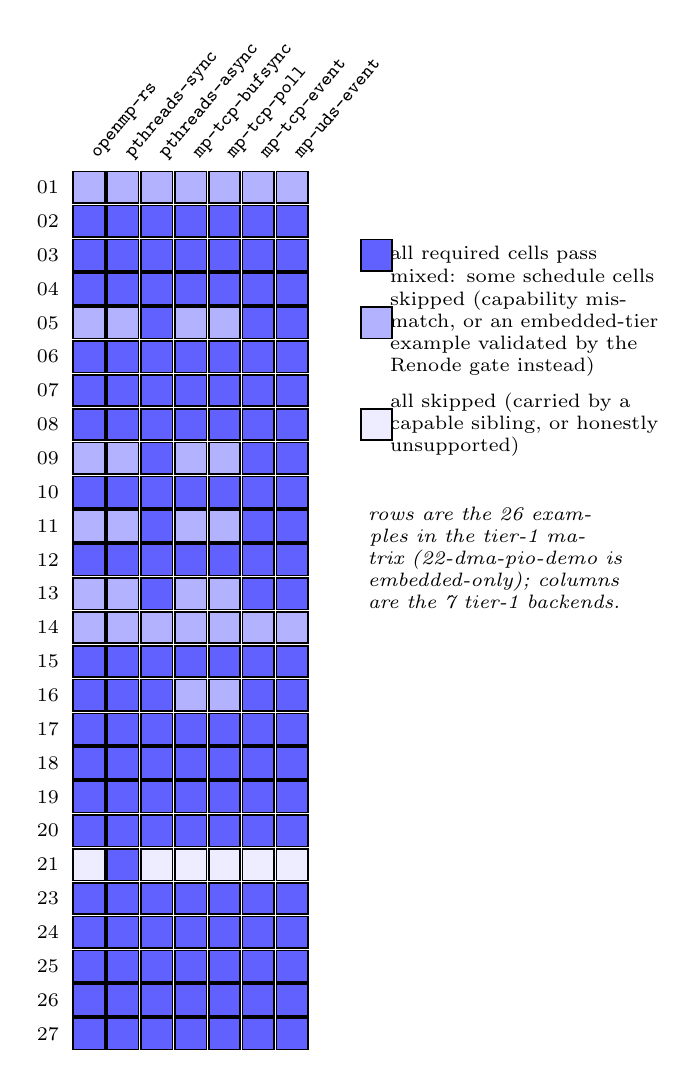
\begin{tikzpicture}[
      x=4.3mm, y=4.3mm,
      cell/.style={draw, semithick, minimum size=4.0mm, inner sep=0pt, anchor=center},
      P/.style={fill=blue!62}, M/.style={fill=blue!30}, s/.style={fill=blue!7},
    ]
    % backend column headers
    \foreach \be [count=\ci from 1] in {%
        openmp-rs, pthreads-sync, pthreads-async, mp-tcp-bufsync,
        mp-tcp-poll, mp-tcp-event, mp-uds-event}
      \node[rotate=50, anchor=west, font=\scriptsize\ttfamily] at (\ci, 0.7) {\be};
    % rows: example label + 7-cell status code (real data)
    \foreach \row/\lab [count=\ri from 0] in {%
        {M,M,M,M,M,M,M}/01, {P,P,P,P,P,P,P}/02, {P,P,P,P,P,P,P}/03,
        {P,P,P,P,P,P,P}/04, {M,M,P,M,M,P,P}/05, {P,P,P,P,P,P,P}/06,
        {P,P,P,P,P,P,P}/07, {P,P,P,P,P,P,P}/08, {M,M,P,M,M,P,P}/09,
        {P,P,P,P,P,P,P}/10, {M,M,P,M,M,P,P}/11, {P,P,P,P,P,P,P}/12,
        {M,M,P,M,M,P,P}/13, {M,M,M,M,M,M,M}/14, {P,P,P,P,P,P,P}/15,
        {P,P,P,M,M,P,P}/16, {P,P,P,P,P,P,P}/17, {P,P,P,P,P,P,P}/18,
        {P,P,P,P,P,P,P}/19, {P,P,P,P,P,P,P}/20, {s,P,s,s,s,s,s}/21,
        {P,P,P,P,P,P,P}/23, {P,P,P,P,P,P,P}/24, {P,P,P,P,P,P,P}/25,
        {P,P,P,P,P,P,P}/26, {P,P,P,P,P,P,P}/27} {
      \node[font=\scriptsize, anchor=east] at (0.4, -\ri) {\lab};
      \foreach \cell [count=\ci from 1] in \row
        \node[cell, \cell] at (\ci, -\ri) {};
    }
    % legend
    \node[cell, P, anchor=west] (lp) at (9.0, -2) {};
    \node[anchor=west, font=\scriptsize] at (9.6,-2) {all required cells pass};
    \node[cell, M, anchor=west] (lm) at (9.0, -4) {};
    \node[anchor=west, font=\scriptsize, align=left, text width=34mm] at (9.6,-4)
      {mixed: some schedule cells skipped (capability mismatch, or an
       embedded-tier example validated by the Renode gate instead)};
    \node[cell, s, anchor=west] (ls) at (9.0, -7) {};
    \node[anchor=west, font=\scriptsize, align=left, text width=34mm] at (9.6,-7)
      {all skipped (carried by a capable sibling, or honestly unsupported)};
    \node[anchor=west, font=\scriptsize\itshape, align=left, text width=34mm]
      at (9.0,-11) {rows are the 26 examples in the tier-1 matrix
      (22-dma-pio-demo is embedded-only); columns are the 7 tier-1 backends.};
  \end{tikzpicture}
  \caption[Tier-1 coverage heatmap]{The tier-1 differential matrix as an
    example-by-backend heatmap (rows are the 26 examples in the tier-1 matrix ---
    \texttt{22-dma-pio-demo} is embedded-only, hence the gap; columns are the
    seven tier-1 backends, of which \texttt{mp-uds-event} uses Unix-domain
    sockets). Each cell aggregates, over an example's schedules, its status on one
    backend: a dark cell (P) means every required schedule passes there, a mid
    cell (M) means some schedule is skipped, and a light cell (s) means all are
    skipped. Of \nmatrixtotal{} declared cells across the seven
    tier-1 backends, \nmatrixpass{} pass (emit, build, run, and reproduce the
    reference byte-for-byte), \nmatrixskip{} are skipped for a recorded reason ---
    the largest group embedded-tier fixtures validated by the simulator gate, the
    rest genuine capability mismatches carried by a capable sibling backend or a
    few honestly-unsupported language shapes --- and none fail. The broad band of
    dark cells is the cross-product of decompositions, IO disciplines, and
    runtimes exercised together on every build.}
  \label{fig:coverage-heatmap}
\end{figure}


The shape of this coverage is what gives the next section its force: it is not a
handful of examples on one backend, but a broad cross-product of decompositions,
IO disciplines, and runtimes, exercised together on every build.

\section{Bit-identity across the tier-1 matrix}\label{sec:res-bitidentity}

The central result is that the seven tier-1 backends agree byte-for-byte. Across
the \nmatrixpass{} passing cells, every backend required for a given example and
schedule reproduces that example's immutable reference output exactly, and the
backends are therefore byte-identical to one another, transitively, through that
shared reference. This holds uniformly across the diversity catalogued in
\cref{sec:val-differential}: the same algorithm under the same schedule produces the
same bytes whether its workers are threads sharing memory, processes exchanging
messages over TCP loopback, or processes over Unix-domain sockets; whether transfers
are synchronous or asynchronous, buffered or unbuffered; and whether the
notification discipline is a blocking receive, a non-blocking poll, or an event
reactor. The decomposition and IO machinery moves the same values to the same
places by the same final ordering, regardless of the runtime mechanism used to do
so. That is the genericity claim, and across the exercised matrix it is not
falsified.

One family of examples is worth singling out because it stresses the part of the
claim most likely to break under reordering. A distributed reduction that combines
per-worker partial results at a host accumulator is only order-independent if the
combining operation is associative and commutative; otherwise the order in which
workers arrive --- which legitimately varies across backends and runs --- would
change the result, and byte-identity would be lost. The system makes the combining
operation explicit --- declared as an attribute on the reducing kernel in the
algorithm (\cref{sec:lang-algorithm}) --- and supports six of them: integer sum,
bitwise or, bitwise xor, minimum, maximum, and bitwise and, each with its correct
algebraic identity element so that the accumulator is initialised soundly. Dedicated examples
exercise the non-trivial cases --- an xor-combined binned reduction, an
integer-minimum reduction whose identity is the type maximum rather than zero, and
the same in floating point. The discipline is enforced rather than assumed: a
floating-point \emph{sum} combine is \emph{rejected at compile time}, because
IEEE-754 addition is not associative and a distributed float-sum could not be made
byte-identical across arrival orders. Refusing the operation is more honest than
silently emitting code that happens to agree on the test input and diverges on
another.

\section{Soundness-gate outcomes}\label{sec:res-soundness}

The soundness gate runs on every build of every cell, so the matrix above is also a
record of the gate's behaviour on hundreds of real, shipping nets. On the committed
corpus the gate rejects nothing: every schedule that is supposed to be sound is
accepted, with no false rejections. This is the outcome a correct gate should
produce on a corpus of correct schedules, and on its own it would be weak evidence
--- an empty check produces the same green build. It is made meaningful by the
negative result alongside it. As described in \cref{sec:val-negative}, the gate's
three properties are each exercised adversarially by a unit test that hands it a
deliberately unsound net: an over-capacity net rejected as a boundedness error, a
stalling net rejected as a deadlock, and a free-choice net rejected as a conflict.
The gate accepts every sound net in the corpus \emph{and} is demonstrated capable
of rejecting unsound ones; both halves are necessary, and both hold. The harness's
own checks --- determinism, the cross-backend differential, and required-coverage
--- are guarded separately by the three injection falsifiers of
\cref{sec:val-negative}, so that no check in the pipeline, static or dynamic, is
trusted on its green result alone.

It bears repeating where the boundary of this result lies. The gate is sound for the
statically-ordered net class the language produces, by exact replay over one firing
order, and is not a general Petri-net model checker (\cref{sec:val-gate}). The
result is ``the gate correctly classifies the nets this system generates,'' not
``the gate decides boundedness for arbitrary nets,'' and the dissertation claims
only the former.

\section{Cluster and embedded value-correctness}\label{sec:res-tiers}

Beyond the tier-1 rig, the cluster and embedded tiers are confirmed to the extent
their runtimes allow, under the compile-mandatory, run-best-effort discipline of
\cref{sec:val-tiers}.

The two MPI backends compile for every schedule they are required to support and,
where a local \texttt{mpiexec} is available, are run and diffed against the same
reference files as the tier-1 backends. On that runtime every exercised MPI cell
reproduces its reference output byte-exactly: the single-program multiple-data
binary, dispatched across ranks, computes the same values as the shared-memory and
loopback backends. The blocking and non-blocking MPI backends thus extend the
byte-identity result from the laptop rig to a distributed-memory runtime, for the
cells exercised. The limit to be clear about is that this is value-correctness on a local
launcher, not a measurement on a production cluster, and that the backends emit
correct point-to-point communication rather than recognising and emitting
collective operations --- a deliberate deferral noted in \cref{sec:be-tier2}.

The embedded tier is confirmed by co-simulation. A standing gate generates the
bare-metal binaries for three multi-microcontroller examples, cross-compiles them
for the embedded target, co-simulates the microcontrollers wired over a virtual
UART fabric, captures the output bytes, and diffs them against the reference file.
All three reproduce their reference output byte-exactly: a two-microcontroller
split-and-add over a 1024-byte payload; the real three-core hearing-aid pipeline,
with heterogeneous front-end, DSP, and RF-controller workers and bidirectional
dataflow, over a 512-byte output; and a two-microcontroller demonstration that
drives two transfers by DMA and one by programmed IO over the same fabric,
again byte-exact over 1024 bytes. The hearing-aid result is the load-bearing one:
it demonstrates that the typed, heterogeneous, multi-worker form lowers all the way
to a real multi-microcontroller system whose per-frame values are correct
end-to-end, including the staged boot-order handling that a bare-metal UART channel
requires and that the hosted tiers never need.

\section{What the falsification rig establishes, and its limits}\label{sec:res-limits}

It is worth stating precisely what these results do and do not establish, because
the value of a falsification rig lies as much in the boundary of its claim as in the
claim itself.

What the rig establishes is this. For the exercised matrix --- twenty-seven
examples, their schedules, and the backends each requires --- the separation of
algorithm, schedule, and target holds to the strongest available standard:
byte-identical output across seven structurally diverse CPU runtimes, extended to a
distributed-memory MPI runtime and to bare-metal multi-microcontroller
co-simulation for the cells those tiers reach. The soundness gate correctly accepts
every sound schedule in the corpus and is demonstrated able to reject unsound nets.
Every check that underwrites these claims has a negative test proving it bites, so a
green result is informative rather than vacuous, and the whole apparatus is
reproducible from a pinned toolchain and a deterministic compiler.

What the rig does not establish is equally important. Byte-identity is shown over
the exercised cells, not proved for all programs the grammar admits; the
specification is exactly as complete as the example corpus, and a shape absent from
the corpus is outside the guarantee. Several such shapes are known and recorded
rather than hidden: a small number of cells are skipped because a language
construct is supported on the single-worker path but not yet on the multi-worker or
cross-backend path --- a data-dependent loop break, of the kind the language's
termination restriction already circumscribes (\cref{sec:lang-limits}), and a
worker-to-worker transfer nested inside a loop body --- and these are reported as
skips with a stated reason, not papered over. The cluster result is
value-correctness on a local launcher, not a cluster-scale measurement, and the MPI
backends emit point-to-point rather than collective communication. The embedded
result covers one reference microcontroller shim; further hardware families are
out-of-tree work. And, as the gate's design requires (\cref{sec:val-gate}), its
soundness guarantee is confined to the statically-ordered net class the
language produces.

The honest summary is that the falsification rig has had every opportunity to refute
the central claim over a broad and diverse matrix, and has not --- while the matrix's
documented edges mark exactly where the claim has not yet been put to the test.
That distinction, between what has survived falsification and what has not been
exposed to it, is the one this chapter is most concerned to keep clear.

\chapter{Discussion}\label{ch:discussion}
% Content cycle: C5. Intent: weigh what the model buys against what it costs,
% honestly. Advantages AND shortcomings get equal billing.

\section{Advantages}\label{sec:disc-advantages}
% Portability for the algorithm class; swappable IO; compile-time soundness;
% falsifiable genericity.

\section{Honest shortcomings}\label{sec:disc-shortcomings}
% The restricted algorithm class (affine/static/single-assignment, no
% scatter, no recursion, no dynamic scheduling); greedy non-optimal schedule;
% single-order soundness scope; integer-only bit-identity and the float-sum
% boundary; check is descriptive, not prescriptive (no cost model); shim
% sprawl; the cost of cluster/HIL CI.

\section{Threats to validity}\label{sec:disc-threats}

\todo{Write Chapter 10 (cycle C5).}

\chapter{Future Work and Open Problems}\label{ch:future-work}

The limitations weighed in \cref{ch:discussion} are not all equal: some are
permanent consequences of the central trade, while others are boundaries the
current system draws conservatively and could move with more work. This chapter is
concerned with the second kind. Each direction below is grounded in a limit the
system actually has, and each is described with an honest estimate of what it would
take and --- crucially --- what it would risk, because several of these extensions
push directly against the static-determinism property that the soundness gate and
the differential rig depend on. A direction that quietly sacrifices that property
would not be an extension of this work but a different system; where that danger
exists, it is named.

\section{Prescriptive scheduling}\label{sec:fw-prescriptive}

The schedule today is hand-written and the compiler is faithful to it; the
\texttt{check} assertions observe whether a bound is met but do nothing to meet it
(\cref{sec:lang-schedule}). The natural next step is to close that loop: turn a
checkable latency assertion into a solved latency budget, so that a schedule states
a goal --- a per-loop latency ceiling, a memory footprint, a worker count --- and
the compiler searches the schedule space for a decomposition that satisfies it.

This is the direction in which the compute-scheduling languages have invested most
heavily, through cost models and autotuners, and the same machinery is applicable
here. But it is genuinely hard, and it changes the contract: a solver needs a cost
model of each target, and a cost model is exactly the thing this work deliberately
does not have, because a faithful one is target-specific and a wrong one would
silently choose bad schedules. A credible version would likely begin narrowly ---
solving for one parameter, such as block size or pipeline depth, against a measured
rather than modelled cost on one target --- and treat full multi-objective schedule
synthesis as a long-term goal rather than a near-term feature. The value of the
present architecture for this work is that the search space is already explicit and
the soundness gate already rejects unsound candidates, so a solver could explore
schedules knowing that every accepted one is sound by construction.

\section{Floating-point determinism}\label{sec:fw-float}

The bit-identity guarantee once stopped at floating-point summation, because IEEE-754
addition is not associative and a distributed float-sum reduced in a varying order
produces varying bytes (\cref{sec:disc-shortcomings}). That boundary has now been
crossed for the cross-backend case, but only partway, and the remaining distance is
worth stating precisely.

What is implemented is the \emph{fixed-order} route: an opt-in \texttt{combine=fsum}
under which the host folds the per-worker partials in a fixed worker-id-sorted order
that is identical on every backend, and the reference oracle reproduces that exact
fold. The reduction lowering, the kernel contract, and the reference implementation
therefore move in lockstep --- the subtlety anticipated below, made concrete --- and a
distributed float sum now carries the same cross-backend byte-identity the integer
combines enjoy, demonstrated across all seven CPU backends by the \texttt{28-bin-fsum}
example. The plain \texttt{sum} combine stays rejected, so the guarantee is opt-in and
the default stays strict.

What remains open is the stronger, \emph{order-independent} route: a reproducible
reduction that computes a fixed result regardless of summation order, for instance by
accumulating into a wide fixed-point superaccumulator --- an integer accumulator wide
enough to represent any partial sum exactly --- that absorbs each addend without
rounding, or by pre-rounding addends to a common
granularity~\cite{demmel2013reproducible}. The fixed-order fold delivered here is
reproducible across backends for a \emph{given} schedule, but it is not the naive
left-to-right IEEE-754 sum, and a different worker count folds the partials
differently --- so it does not yet give ``same bytes across schedules.'' An
order-independent scheme would close that gap, making every decomposition agree
bit-for-bit on a single reproducible result independent of worker count (the result
being the scheme's own --- the exact sum for a superaccumulator, the pre-rounded sum
for pre-rounding --- not necessarily the naive single-pass IEEE sum). The subtlety that
made even the fixed-order step less self-contained than it first appears --- that the
immutable oracle, the rig's trust anchor, must adopt the same scheme so cross-backend
agreement is also agreement with the oracle --- applies with full force to the
order-independent route, and is the reason it is the higher-value but heavier
remaining direction: it lifts the schedule-invariance limit that still excludes part
of a whole numerical domain, but it is not the trivial drop-in the opt-in framing
alone would suggest.

\section{Beyond the affine, static class}\label{sec:fw-affine}

The hardest and most consequential limits are the ones that define the algorithm
class itself, and they come in several grades of difficulty.

\paragraph{Distributed gather and scatter.} Data-dependent indexing is supported
today only conservatively: a gather broadcasts the whole indexed array and a
scatter replicates and recombines its target, and a scatter onto an affine-
partitioned target is rejected (\cref{sec:arch-transfer}). A precise distributed
gather/scatter --- one that moves only the elements a worker actually touches ---
would require a communication-synthesis pass that reasons about the index array's
contents, which are not known at compile time, and so would need either a runtime
exchange phase or a two-pass inspector/executor scheme --- a first pass that
inspects the index array to plan the communication and a second that executes that
plan --- of the kind sparse libraries use~\cite{saltz1991runtime}. This is well-trodden ground in distributed sparse computing, but importing it
here means admitting a runtime-determined communication pattern, which sits in
tension with the static firing order. The difficulty is sharper than the
bounded-iteration case treated below in this section. Bounded data-dependent
\emph{iteration} (the capped \texttt{until} loop exercised by
\texttt{21-jacobi-converge} and \texttt{29-jacobi-cap-hit}) works because its only
runtime unknown is a scalar trip count: a compile-time cap fixes the worst-case
firing order and any shorter run replays as a sub-trace of it. A precise
gather/scatter's runtime unknown is not a scalar but an entire address map --- which
element moves to which worker --- whereas the soundness gate replays a communication
structure fixed at compile time. The only compile-time-fixed structure that covers
every possible index pattern is the conservative whole-array broadcast the backends
already emit; that broadcast is, in effect, the trivial statically sound envelope,
merely an untightened one. Tightening it is therefore not blocked by bounding the
exchange's \emph{size} --- that bound is the part the iteration work already
demonstrates --- but by deciding \emph{which} elements move while the gate still sees
a fixed structure. Closing the gap needs either a gate that admits a bounded family
of runtime communication patterns or a static envelope provably sound for any pattern
yet tighter than whole-array; both are verification advances the present soundness
argument does not reach, which is why the conservative broadcast remains the only
sound option today.

\paragraph{Data-dependent control flow.} Convergence-driven termination --- a loop
that runs ``until converged'' --- is the single most-requested capability the model
still lacks in general, and lifting it \emph{fully} is the deepest change, because an
unbounded data-dependent trip count means the firing order is no longer statically
determined, which is the property everything else rests on. The bounded middle path,
however, is no longer hypothetical. Bounded data-dependent iteration --- a loop with a
compile-time maximum trip count and a runtime early exit, so the worst-case firing
order remains statically analysable even though the actual run may stop early --- is
\emph{realized on the single-worker path}. Two corpus examples
(\texttt{21-jacobi-converge} and \texttt{29-jacobi-cap-hit}, the optional
\texttt{until} clause of \cref{app:grammar}) compile and run a Jacobi convergence
loop value-correctly: one exits early, and one runs the full cap so the worst-case
bound the soundness gate analyses is itself an exercised, byte-identical execution
path rather than an assertion. This holds because the gate replays the full capped
unroll and any early exit is a sub-trace of it (soundness preserved by the cap), and
because the exact-integer halt predicate is a deterministic, backend-agnostic
function of the data, so every backend stops at the same generation (the differential
test preserved). Two residuals remain. First, the break is single-worker only: on the
multi-worker path the convergence scalar is a cross-worker reduction, so the early
exit must become a collective all-reduce-and-broadcast at a barrier --- every worker
branching on the identical global value and exiting at the same generation by
construction --- which keeps the firing order static but is a genuinely new collective
pattern not yet built; multi-worker convergence cells are recorded as skips meanwhile.
Second, byte-identity is at risk under a \emph{floating-point} convergence predicate,
whose comparison value depends on accumulation order, tying this direction back to the
float-determinism limit above. Even so, the realized form already admits a useful
subset of single-worker iterative solvers --- those with a known iteration cap and an
exact termination test --- and the residual is a bounded, well-scoped lift rather than
the open-ended problem unbounded data-dependent control flow poses.

\paragraph{Sparse iterative solvers.} A full sparse solver needs both of the
above --- data-dependent indexing and convergence-driven termination --- which is
why it sits entirely outside the present model. It is listed here not as a
near-term target but as the natural destination if the two preceding directions
both succeed, and as an honest marker of how far the current class is from
general numerical computing.

\paragraph{Precise inference, and the remaining halves of the region saving.} The
groundwork here is now partly built, which sharpens what is left to do. The backends
already transmit only the inferred region on a cross-worker edge whose region is a
single contiguous span, cutting wire volume measurably (\cref{sec:res-quant-comm}); two
distinct extensions remain, one on the inference side and one on the backend side, and
they are independent. On the inference side, the transfer-inference pass still degrades
to whole-array broadcast whenever an index is not an affine, contiguous function of the
partition variables. A polyhedral analysis, using an established integer-set library,
could compute precise transferred regions for a broader class of affine and
piecewise-affine index expressions than the current prefix-based inference handles,
without changing the language --- and because the wire now follows the inferred region,
a sharper inference would directly narrow more edges rather than merely improving
receiver-side correctness. On the backend side, two cases the wire flip deliberately
left whole-array remain: a \emph{strided} or non-prefix region (a column band of a
row-major matrix, an irregular halo) needs a banded pack-and-scatter the backends do not
yet emit, and the embedded tier needs a banded receive to match a banded send. And the
\emph{footprint} half is wholly untouched: every worker still allocates the array
full-shaped and pastes its received span into place, so per-worker memory is unchanged;
reducing the allocation to the owned band needs index rebasing at kernel-call sites or a
banded-view abstraction, because downstream reads index with global coordinates
(\cref{sec:disc-shortcomings}). All of these are internal precision improvements that
risk nothing in the guarantees --- the firing order, the soundness gate, and the
byte-level results are unchanged, only the volume moved and the memory held --- which
keeps the direction comparatively safe, but it is a several-part one, of which only the
contiguous-span wire flip is so far done.

\section{New target tiers}\label{sec:fw-tiers}

The three tiers --- commodity CPU, message-passing cluster, embedded
microcontroller --- cover a wide span but stop short of massively parallel
accelerators. A GPU or neural-processing-unit tier is a plausible fourth, and the
event contract is in principle agnostic enough to drive one. But the fit is not
free: a GPU's execution model is bulk-synchronous (alternating compute phases with global
synchronisations across many parallel threads) over thousands of lanes, with a
memory hierarchy the current contract does not model, and the \texttt{Alloc} and
\texttt{Free} events (\cref{sec:arch-petri}), currently reserved in the event
contract but emitted by no backend, would have to become load-bearing to place data
across that hierarchy. The honest assessment is that a
GPU tier is a research project in its own right, not a matter of writing one more
shim, and that claiming the architecture ``extends to GPUs'' without having done it
would be exactly the kind of overclaim this document has tried to avoid. It is
listed as an open direction, not a promised one.

The cheaper and more certain tier work is further breadth within the existing
embedded tier. A second microcontroller family has already been added --- an
nRF52840 (Cortex-M4F) shim whose UARTE EasyDMA transmit is a genuinely different
register interface from the STM32 USART --- byte-exact on the same examples
(\cref{ch:results}), which both demonstrates the hardware-abstraction trait is a
real portability seam and calibrates the cost: that second family reused the generic
backend and the test harness unchanged, swapping only the concrete shim, the memory
map, and one linker flag, because it shared the Cortex-M target the toolchain
already builds and had a ready simulator model. Additional families --- each a
separate shim against the committed trait --- would broaden the evidence further.
This is bounded, well-specified engineering rather than research; cheap when a family
shares the target and has a simulator model, more expensive when it needs a new
target triple or a model that does not yet exist. It remains the most direct way to
widen the part of the claim that \cref{sec:disc-shortcomings} identifies as the
narrowest.

\section{A quantitative performance and scaling study}\label{sec:fw-quant}

This document confined its main results to correctness and coverage, because the
contribution it defends is the separation and its falsifiability, not the speed of
the emitted code (\cref{ch:results}). It does report a set of \emph{static}
engineering characteristics --- per-backend code footprint, generated-code size, and
how the soundness gate's analysis net scales with problem size
(\cref{sec:res-quant}) --- so the cost of the genericity is at least described. Two
quantitative directions remain genuinely open, and it is worth stating each
precisely.

The first is a \emph{runtime} performance and scaling study: how the emitted
programs' wall-clock time varies with worker count, schedule, and backend on real
hardware --- and, for the cluster tier, on an actual cluster rather than a local
launcher. This is the measurement that would turn the portability claim from ``the
same values everywhere'' into ``the same values, and here is what each decomposition
costs,'' and it is the input the prescriptive-scheduling direction of
\cref{sec:fw-prescriptive} would need. It is deliberately deferred here because a
credible runtime study demands a benchmarking methodology --- worst-case inputs,
controlled hardware, warm-up and variance discipline --- that is a project in itself,
and because no runtime number bears on the correctness claims already established: a
slow but byte-identical program still falsifies nothing.

A scoping observation explains why this was, until recently, more than a matter of
securing time on a cluster, and it once coupled the runtime study tightly to the
gate-scaling direction below. At the corpus's problem sizes the emitted programs'
wall-clock is dominated by fixed per-invocation overhead rather than by computation ---
a single-worker matrix multiply at the corpus dimension finishes in about a
millisecond, of which the few thousand integer multiply--adds account for only
microseconds; the remainder is process spawn, input loading, and thread setup, not
arithmetic --- so a meaningful scaling signal emerges only at substantially larger
problem sizes. The gate is not separable from the build: there is no option to emit a
decomposed program without analysing it, so the cost of compiling the decompositions
one would want to time used to bound what could be timed at all. That coupling has now
loosened for the dominant case. The gate proves the single-shot matched-pair
communicating subclass --- which is the shape of most of the corpus's distributed
schedules --- symbolically, so building the four-worker distributed matrix multiply at
$N=512$ now costs about 7.2\,megabytes of compiler memory rather than the hundred-plus
gigabytes its expanded net would project (\cref{sec:res-quant-net}). One can therefore
now compile exactly those large distributed decompositions, which removes the gate as
the binding obstacle to timing them. What remains coupled is narrower: the loop-carried
and pipelined distributed shapes still expand, so a runtime study that needed to scale
\emph{those} specific schedules would still wait on the gate work below. A credible
runtime study therefore now waits primarily on a representative cluster and a
disciplined methodology rather than on the compiler --- except for the residual
loop-carried and pipelined shapes, where the two open problems remain coupled.

The second direction is the gate-scaling limitation that \cref{sec:res-quant-net}
measured, and it has been \emph{substantially} closed, in two steps. Because the
soundness gate replayed a net expanded over the iteration space --- roughly one place and
one transition per kernel firing --- its cost was linear in the number of firings, cheap
for the corpus but unable to scale to a problem with billions of firings. First, for the
\emph{buffer-free} subclass (a single worker, or any schedule with no cross-worker
transfer) the gate now reasons about the \emph{looped} structure directly: it proves
soundness from the rolled ACFG in time independent of the iteration count, never building
the expansion. Second, and the harder step, the symbolic proof now reaches across a
cross-worker boundary, to the \emph{single-shot matched-pair} communicating subclass: a
distributed schedule whose every transfer is one \texttt{Push} matched by one
\texttt{Wait} at loop depth zero, so the shared buffer place's peak occupancy is provably
one and at most its capacity. This is the dominant distributed shape --- the corpus's
distributed reductions, stencils, matrix multiply, sparse mat--vec, histogram, and
scatter all fall in it --- and proving it symbolically, against a firing-order invariant
pinned by property tests and cross-checked against the expanded replay on every gated
cell, is what keeps the $N=512$ distributed matmul compile flat. What remains open is the
\emph{loop-carried} and \emph{pipelined} communicating shapes --- a transfer whose buffer
occupancy depends on cross-iteration drainage, or one that deliberately keeps several
frames in flight --- whose boundedness still depends on a firing-order interleaving the
symbolic analysis does not yet cover. A steady-state occupancy argument over their looped
\texttt{Push}/\texttt{Wait} structure is the concrete compiler work still outstanding. It
is deliberately not approximated: an imprecise buffer analysis could accept a net the
expanded replay would reject, trading soundness for scaling, which the gate's whole
purpose forbids --- so anything outside the proven subclasses is routed loudly to the
sound expanded replay until the symbolic argument is extended to it too.

Taken together, these directions share a common discipline: each is judged not only
by what it would add but by what it would risk to the determinism the system is
built on. Two of them sit off that risk axis entirely --- prescriptive scheduling
and the quantitative study change no guarantee, the first being an optimisation
question and the second an empirical one. Of the rest, the order-independent float
reduction and the polyhedral precision improvement add capability without touching
the guarantees, even though the polyhedral work is grouped, by topic, inside the
affine-class section; bounded data-dependent iteration and a precise distributed
scatter push against the static firing order and must be done carefully if at all;
and unbounded data-dependent control flow and a GPU tier would, if done naively,
dismantle the very properties that make the present system worth having. The
interesting future work is therefore not simply to lift the limits, but to lift them
while keeping the soundness gate sound and the differential test meaningful --- which
is the same constraint that shaped the original design.

\chapter{Conclusion}\label{ch:conclusion}

This dissertation began with a narrow, concrete complaint: that porting a parallel
algorithm across CPU threads, a message-passing cluster, and an embedded
microcontroller means rewriting it, because the decomposition and the IO --- not the
arithmetic --- are written by hand and tangled into the source, separately for each
target. Compute scheduling has long had first-class language support; IO scheduling
has not. The work set out to give it that support and to make the resulting
separation claim something stronger than a design aspiration.

The contribution is best stated soberly. The system rests on a strict separation
between an algorithm sublanguage, which says what to compute and contains no worker,
buffer, transport, or synchronisation, and a schedule sublanguage, in which
decomposition, IO semantics, and target are first-class directives the algorithm
never sees. The two are unified by a single Petri-net intermediate representation
that carries transfer synthesis, synchronisation, and a compile-time soundness gate
together, so that boundedness and deadlock-freedom are reported as compile errors
rather than discovered as runtime hangs. And the genericity claim is made
mechanically falsifiable by a cross-backend differential test: the same algorithm,
under every schedule and capable backend, must produce byte-identical output, and
any leak across the algorithm/schedule or middle-end/presentation boundary that
makes two backends diverge turns that test red. The implementation drives
twenty-seven worked algorithms through ten
backends across three tiers --- seven commodity-CPU backends, two message-passing
cluster backends, and one embedded backend with multi-microcontroller co-simulation.

What was demonstrated is correspondingly bounded. The seven CPU backends agree
byte-for-byte across the exercised schedule-by-backend matrix; the soundness gate
accepts every sound schedule in the corpus and is shown, by adversarial tests, able
to reject unsound nets; every check that underwrites these claims has a negative
test proving it can fail, so a green result is informative rather than vacuous; and
the cluster and embedded tiers are confirmed to value-correctness on a local
message-passing launcher and to byte-exact co-simulation respectively. None of this
is a proof that every program the grammar admits is byte-identical everywhere; it is
the result of a falsification rig that has had every opportunity over a broad and
diverse corpus to refute the central claim and has not, with its documented edges
marking exactly where the claim has not yet been tested.

The work is equally clear about its price. The whole architecture is bought with a
single trade --- expressiveness for a statically determined, deterministic firing
order --- and that trade defines a real boundary. The algorithm class is affine,
static, single-assignment, and integer-valued, with floating-point summation
excluded by the determinism it would break; there is no data-dependent control flow,
no recursion, and no dynamic scheduling; the schedule is checked, not optimised, and
carries no cost model; the soundness guarantee is scoped to coordination within a
restricted net class, not to value-correctness or to arbitrary nets; and the cheap
CPU tier carries the strongest form of the formal claim while the more exotic tiers
are confirmed more narrowly. These are consequences of the central commitment, not
oversights, and the dissertation has tried throughout to weigh them with the same
seriousness as the advantages.

The bet the work makes is that for a particular and not uncommon audience --- people
moving regular, deterministic algorithms across heterogeneous parallel and embedded
targets, who value portability and provable coordination over peak performance and
can live within the affine, static class --- a system that makes IO a first-class
schedule concern, decides soundness at compile time, and renders its genericity
claim falsifiable is worth more than a more expressive system whose portability is
asserted rather than tested. Whether that bet generalises beyond the demonstrated
class is the substance of the future work --- including order-independent
floating-point reduction, bounded data-dependent iteration, precise distributed
communication, further hardware families, prescriptive scheduling, and the deferred
runtime performance study --- each of which would widen the audience or sharpen the
evidence. The discipline that
shaped the original design --- lift a limit only while keeping the soundness gate
sound and the differential test meaningful --- remains the constraint under which
that widening must happen.

The smallest honest summary is this. The expensive part of portable parallel
software is not the arithmetic; it is the decomposition and the IO. This work
factored those out into a separate, swappable schedule, unified them in one analysable
representation, and then --- rather than asking to be believed --- built the
instrument that would expose the separation if it leaked, and ran it on every build.
Across the corpus, it did not leak. That is a modest claim, precisely scoped, and it
is the one the dissertation stands behind.


\appendix
\chapter{Example Catalogue}\label{app:examples}
% Content cycle: C5. Intent: tabulate the driving examples and what each
% stresses (the test suite that is the specification).

\todo{Catalogue the driving examples and the property each one exercises
(cycle C5).}

\chapter{The \nuclang{} Grammar}\label{app:grammar}
% Content cycle: C5. Intent: the algorithm and schedule sublanguage grammars.

\todo{Give the algorithm and schedule sublanguage grammars (cycle C5).}

\chapter{Capability Matrix}\label{app:capability-matrix}
% Content cycle: C5. Intent: the full backend capability matrix.

\todo{Tabulate the full backend capability matrix (cycle C5).}

\chapter{Reproducibility}\label{app:reproducibility}
% Content cycle: C5. Intent: how to build and run the compiler, the example
% matrix, and this dissertation, from a pinned environment.

\todo{Document the pinned build/run instructions for the compiler, the
example matrix, and this document (cycle C5).}


\backmatter
\printbibliography[heading=bibintoc]

\end{document}
